\documentclass[10pt, a4paper]{article}

\usepackage[a4paper, top=0.5cm, bottom=0.5cm, left=0.5cm, right=0.5cm, landscape]{geometry}
\usepackage{mathtools}
\usepackage{amsfonts}
\usepackage{multicol}
\usepackage{setspace}
\usepackage{graphicx}
\usepackage[dvipsnames]{xcolor}


\author{Zachary Chua Yan Ern}
\date{16 September 2020}
\setstretch{1.25}

\newcommand{\highlight}[1]{{\color{red}\textbf{#1}}}
\newcommand{\blue}[1]{{\color{MidnightBlue}#1}}
\newcommand{\red}[1]{{\color{red}#1}}
\newcommand{\green}[1]{{\color{ForestGreen}#1}}

\begin{document}
	\scriptsize %tiny
	\setlength\parindent{0pt}
	\setlength{\columnseprule}{0.1pt}
	
	\begin{center}
		{\large CS2100 CheatSheet}\\
		by Zachary Chua
	\end{center}
	
	\begin{multicols*}{3}
		
		{\normalsize\textbf{C programming}}\\
		
		\textbf{Data Types}\\
		1. int (integer): 4 bytes, -2,147,483,648 $(-2^{31})$ to 2,147,483,647 $(2^{31} - 1)$\\
		2. float (real number): 4 bytes\\
		3. double (real number): 8 bytes\\
		4. char (character): 1 byte, enclosed in pair of single quotes eg. 'a'\\
		
		\textbf{Preprocessor Directives}\\
		1. Include libraries eg. \texttt{\#include <math.h>}, need to compile with \texttt{-lm} if imported math lib\\
		2. Macro expansions eg. \texttt{\#define PI 3.142 //use CAPS for macro}
		Macro expansions do a textual substitution\\
		
		\textbf{Input/Output}\\
		Input/Output statements:\\
		- scanf( format string, input list );\\
		- printf( format string );\\
		- printf( format string, print list )\\
		Format Specifiers\\
		
		\begin{tabular}{ | c | c | c |}
			\hline
			Placeholder & Variable Type & Function Use \\
			\hline
			\%c & char & printf / scanf\\
			\hline
			\%d & int & printf / scanf\\
			\hline
			\%f & float or double & printf \\
			\hline
			\%f & float & printf \\
			\hline
			\%lf & double & scanf \\
			\hline
			\%e & float or double & printf (for scientific notation)\\
			\hline
		\end{tabular}\\
	
		Examples\\
		- \%5d: displays integer with width 5, right justified\\
		- \%8.3f: display real number, width of 8, 3dp, right justified\\
		
		\textbf{Operators}\\
		\textbf{Equals operator}\\
		= has the side effect of returning the value assigned\\
		
		\textbf{Arithmetic Operators and Precedence}\\
		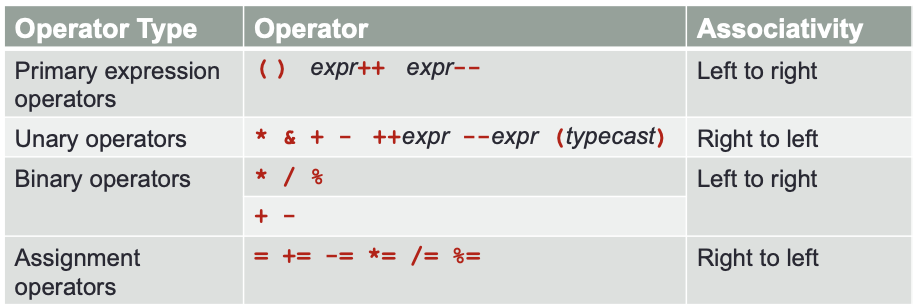
\includegraphics[scale= .5]{./assets/arithmeticOperators}\\
		Mixed-Type Arithmetic Operations\\
		- \texttt{int m = 10/4;} means \texttt{m = 2;}\\
		- \texttt{float p = 10/4;} means \texttt{p = 2.0;}\\
		- \texttt{int n = 10/4.0} means \texttt{n = 2;}\\
		- \texttt{float q = 10/4.0} means \texttt{q = 2.5;}\\
		- \texttt{r = -10/4.0;} means \texttt{r = -2;}\\
		
		\textbf{Type Casting}\\
		syntax: \texttt{ (type) expression }\\
		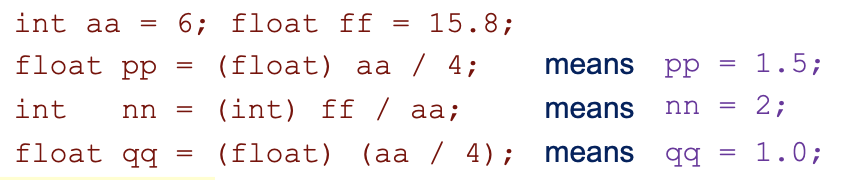
\includegraphics[scale= .5]{./assets/typeCast}\\
		
		\textbf{Remainder}\\
		\% is remainder in C\\
		- \texttt{a = 10 \% 4} $\rightarrow$ \texttt{a = 2}\\
		- \texttt{a = -10 \% 4} $\rightarrow$ \texttt{a = -2}\\
		
		\textbf{Booleans}\\
		No boolean types in C, use integers ie\\
		- 0 represents false\\
		- any other integer (usually 1) represents true\\
		
		\textbf{Operator Precedence}\\
		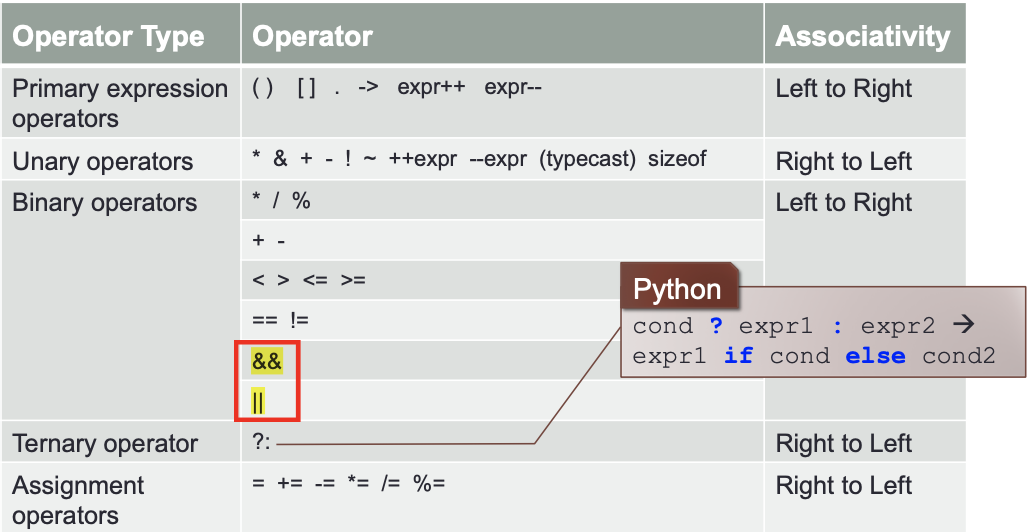
\includegraphics[scale= .5]{./assets/logicOperators}\\
		\highlight{Note} that precedence of $\&\&$ is greater than that of $||$\\
		$\&\&$ and $||$ use short-circuit evaluation\\
		
		\textbf{Loops}\\
		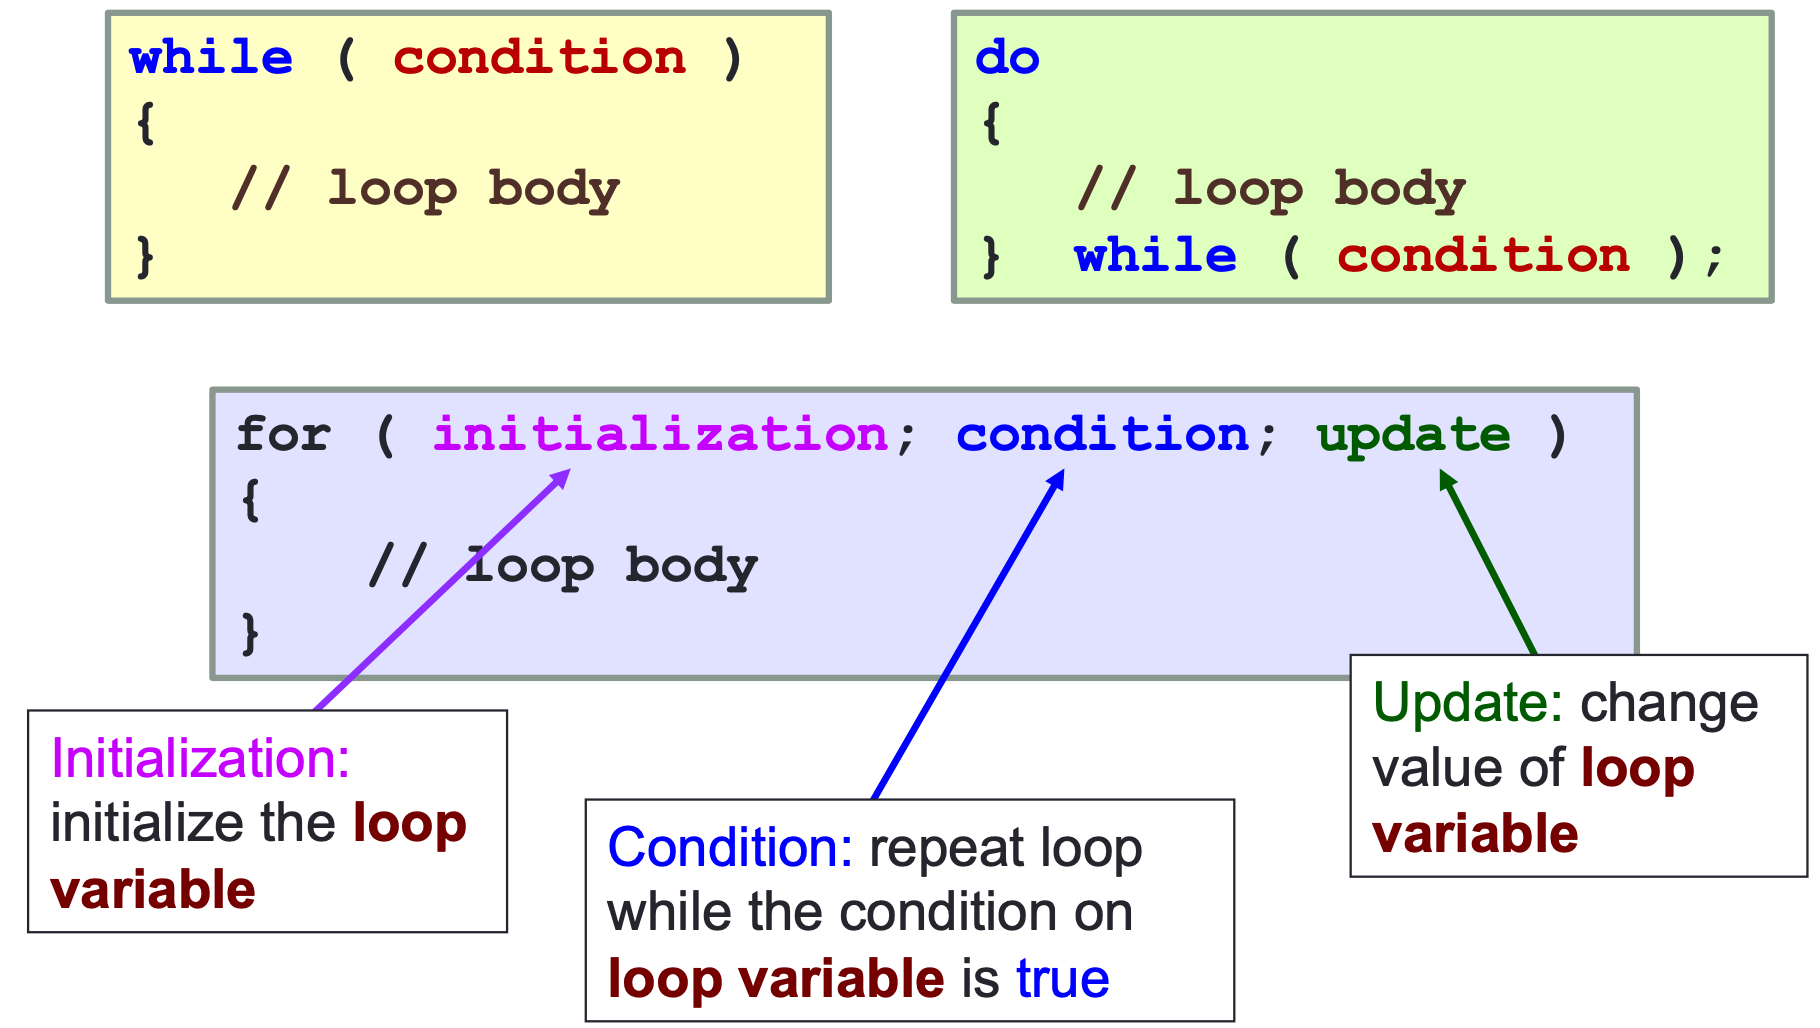
\includegraphics[scale=0.23]{./assets/loops}\\
		For \texttt{for} loops in C, declaration of the loop variable has to be before the \texttt{for} loop\\
		{\normalsize\textbf{Number Systems}}\\
		\textbf{Data Representation}\\
		- bit: 0 or 1\\
		- byte: 8 bits\\
		- word: Multiple of bytes, 4 for mips\\
		$N$ bits can represent up to $2^N$ values, from $0 - (2^N - 1)$\\ 
		To represent $M$ values, $\lceil{log_2^M}\rceil$ bits are required\\
		In C,\\
		- Prefix 0 for octal, eg $032$ represents $(32)_8$\\
		- Prefix 0x for hexadecimal, eg $0x32$ represents $(32)_16$\\
		
		\textbf{Convertion from Decimal to Base $R$}\\
		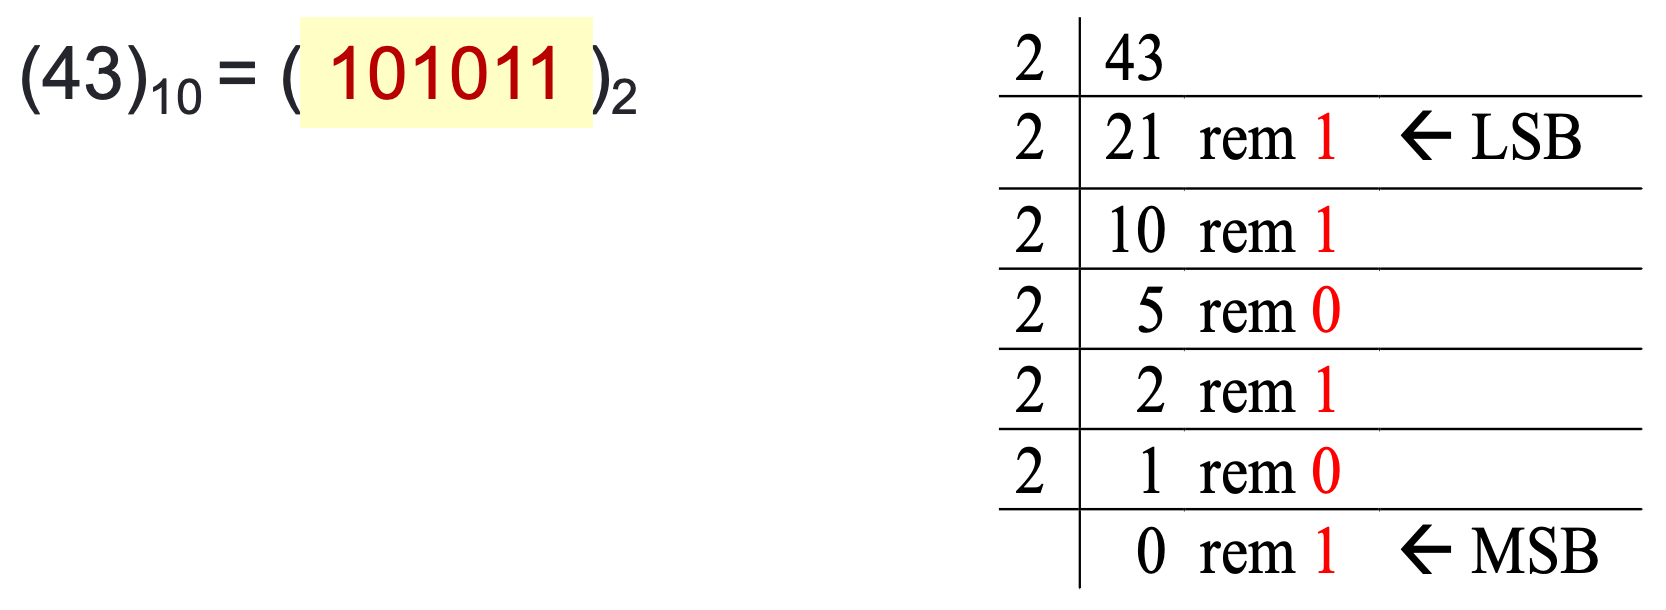
\includegraphics[scale=0.25]{./assets/baseConversion}\\
		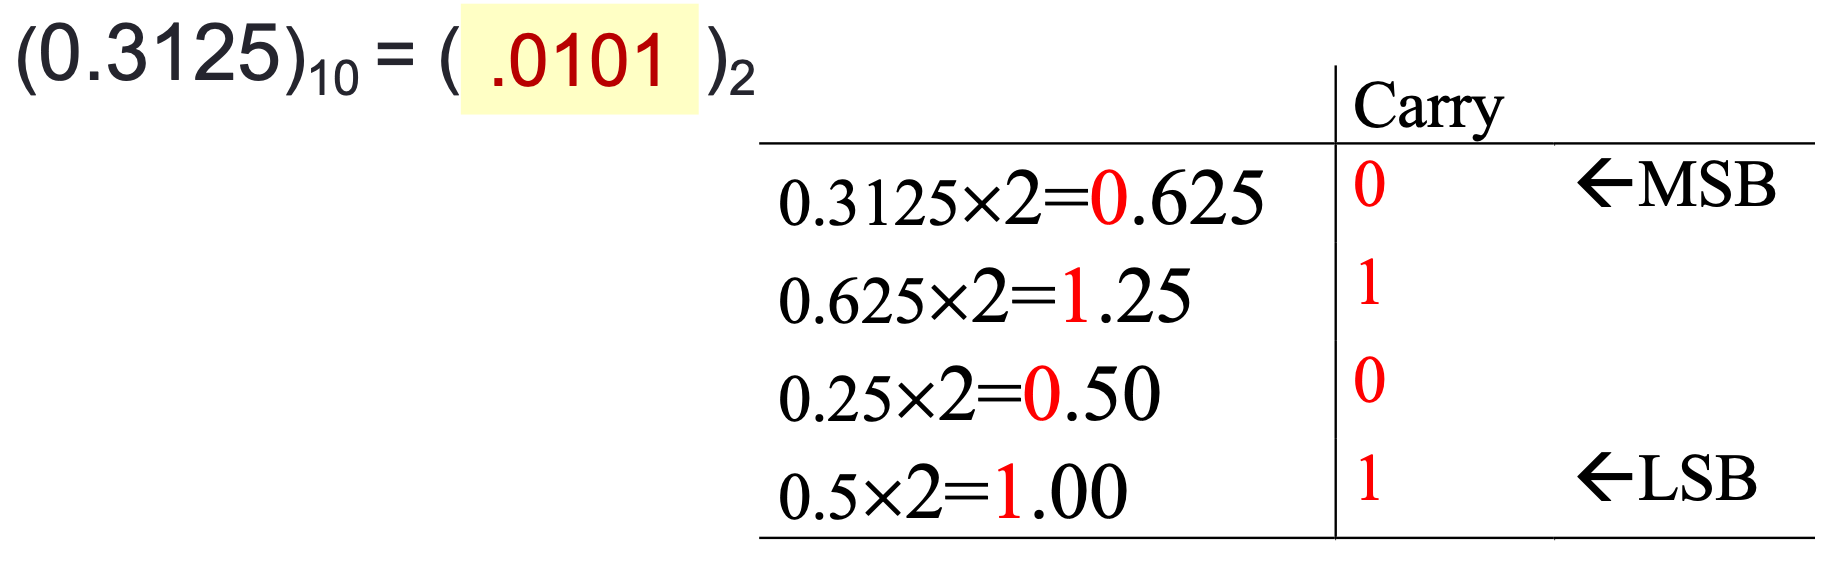
\includegraphics[scale=0.25]{./assets/baseConversion2}\\
		
		\textbf{Binary to Octal and Hexa shortcuts}\\
		- Binary to Octal: partition in groups of 3, take the value of the groups\\
		- Octal to Binary: reverse
		- Binary to Hexa: partition in groups of 4, take the value of the groups\\
		- Hexa to Binary: reverse, convert hexa to binary, extend to 4 digits if needed\\
		
		\textbf{ASCII code}\\
		Integers $(0 - 127)$ and characters are 'somewhat' interchangeable in C\\
		
		\textbf{Negative Numbers}\\
		3 representations\\
		1. Sign-and-Magnitude\\
		2. 1s complement\\
		3. 2s complement\\
		
		\textbf{Sign and Magnitude}\\
		Sign is represented by sign bit; 0 for $+$ and 1 for $-$\\
		First bit is sign bit, other 7 bits are read as normal\\
		- Largest value: $2^{n - 1} - 1$\\
		- Smallest value: $-2^{n - 1} + 1$\\		
		- 2 zeroes: $+0 = 00000000$ and $-0 = 10000000$\\
		- Range: $2^{n - 1} - 1$ to $-2^{n - 1} + 1$\\
		To negate the number, just invert sign bit\\
		
		\textbf{1s Complement}\\
		Negated value of $x$ is given by $-x = 2^n - x - 1$\\
		- Largest value: $2^{n - 1} - 1$\\
		- Smallest value" $- 2^{n - 1} - 1$\\
		- 2 Zeroes: $+0 = 00000000$ and $-0 = 11111111$\\
		- Range: $-(2^{n - 1} - 1)$ to $2^{n - 1} - 1$\\
		To negate a number, invert all bits\\
		\highlight{Note} that the first bit still represents the sign: 0 for positive and 1 for negative.\\
		
		\textbf{2s Complement}\\
		Negated value of $x$ is given by $-x = 2^n - x$\\
		- Largest value: $2^{n - 1} - 1$\\
		- Smallest value: $-2^{n - 1}$\\
		- Range: $-2^{n - 1}$ to $2^{n - 1} - 1$\\
		To negate a number, invert all bits, then add 1\\
		For fractions same thing, flip then add one to LSB\\
		\highlight{Note} that MSB still represents the sign, and that MSB "has a value" of $-2^{n - 1}$\\
		
		\textbf{Sign Extension}\\
		For 1s and 2s complement: Extend sign bit\\
		For SaM: Pad 0s after the sign bit\\
		
		\textbf{Arithmetics}\\
		\textbf{2s Complement Addition and Subtraction}\\
		Algorithm for adding integers $A$ and $B$\\
		1. Perform binary addition on the two numbers\\
		2. Ignore the carry out of MSB\\
		3. Check for overflow, overflow occurs if the 'carry in' and 'carry out' of the MSB are different. Or if the result is opposite sign of $A$ and $B$\\
		
		\textbf{1s Complement Addition and Subtraction}\\
		Algorithm for adding integers $A$ and $B$\\
		1. Perform binary addition on the two numbers\\
		2. If there is a carry out of the MSB, add 1 to the result (at the LSB)\\
		3. Check for overflow\\
		
		\textbf{Overflows}\\
		Overflows are a result of addition/subtraction going beyong the range of numbers\\
		- positive add positive $\rightarrow$ negative\\
		- negative add negative $\rightarrow$ positive\\
		
		\textbf{Excess Representation}\\
		Allows the range of values to be distributed evenly between positive and negative values, using a simple translation (subtraction)
		\begin{center}
			Excess representation = Value + excess
		\end{center}
		eg for excess-8, rep = Value + 8\\
		For 4-bit  numbers, usually use excess-7 or excess-8\\
		
		\textbf{Real numbers}\\
		
		\textbf{Fixed point representation}\\
		Number of bits allocated for whole number part and fractional part are fixed\\
		- Advantage: Easier computation\\
		- Disadvantage: smaller range for a given precision\\		
		
		\textbf{Floating point representation}\\
		IEEE 754 Floating-Point Representation\\
		3 components: sign, exponent, mantissa (fraction)\\
		Similar to standard form\\
		Radix is assumed to be 2\\
		1. Single Precision (32-bit): 1-bit sign, 8-bit exponent with excess-127, 23-bit mantissa\\
		2. Double Precision (64-bit): 1-bit sign, 11-bit exponent with excess-1023, 52-bit mantissa\\
		Mantissa normalised with an implicit leading bit 1\\
		eg. -6.5 in decimal
		\begin{center}
			$-6.5_{10} = -110.1_2 = -1.101_2 * 2^2$\\
			IEEE 754: 1 10000001 10100000000000000000000$_2$ = C0D00000$_{16}$\\
		\end{center}
		
		{\normalsize\textbf{Pointers and Functions}}\\
		\textbf{Pointers}\\
		Can refer to the address of a variable by usiing the \textit{address of operator}, \&\\
		\%p is used as the format specifiier for addressses, addresses are printed out in hexadecimal format\\
		
		\textbf{Pointer Variables}\\
		Variable that contains the address of another variable.\\
		
		\textbf{Declaring a Pointer}\\
		Syntax:
		\begin{center}
			\texttt{type *pointer\_name}\\
		\end{center}
		- pointer\_name is the name of the pointer (Good practice to name a pointer with suffix \_p or \_ptr)\\
		- type is the data type of the variable this pointer may point to\\
		eg. \texttt{int *a\_ptr} declares a pointer to an int named \texttt{a\_ptr}\\
		
		\textbf{Assigning Value to a Pointer}\\
		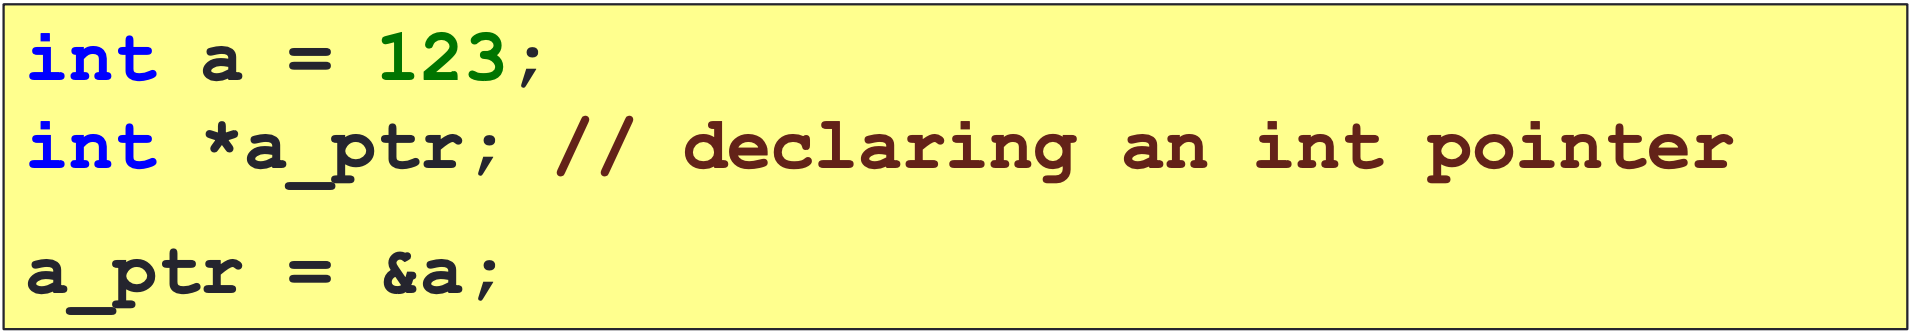
\includegraphics[scale=0.25]{./assets/pointerDeclaration}\\
		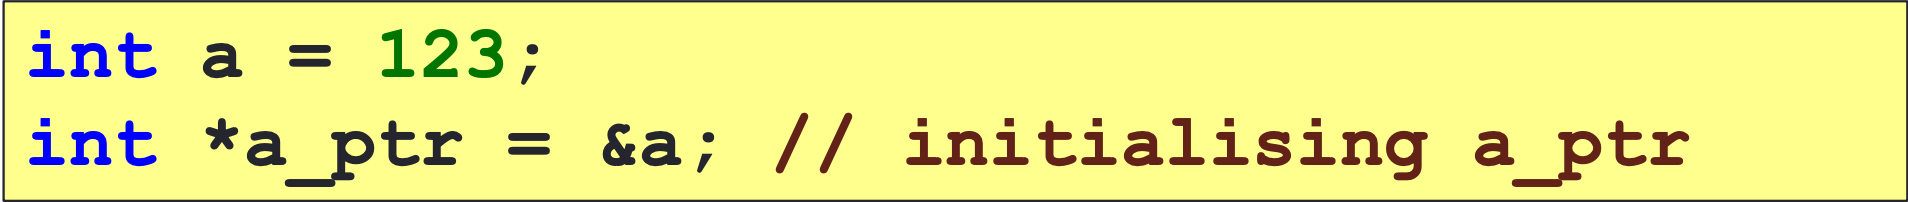
\includegraphics[scale=0.25]{./assets/pointerDeclaration2}\\
		
		\textbf{Accessing Variable through Pointer}\\
		Once a\_ptr points to a, can access a through a\_ptr using \textit{indirection operator}, (or dereferencing operator) *\\
		ie. a\_ptr* === a\\
		
		\highlight{Note} that\\
		- \texttt{int *a\_ptr} is a declaration of a pointer to an int with the name a\_ptr\\
		- \texttt{*a\_ptr} is the value AT the address stored in a\_ptr\\
		
		\textbf{Incrementing Pointers}\\
		Incrementing a pointer means that the pointer will look at the NEXT chunk of data,\\
		ie. incrementing an int/ float ptr increases value by 4, incrementing a char ptr increases value by 1, incrementing double ptr increases value by 8\\
		
		\highlight{Note} remember to assign the pointer variable an address before using if not it would be pointing somewhere unknown\\
		
		\textbf{User Defined Functions}\\
		Function Definitions follow the following syntax
		\begin{verbatim}
			return_type name(p1_type p1_name, p2_type p2_name, ...) {
				    // function body
			}
		\end{verbatim}
		Function prototypes follow the following syntax (names of params not needed)
		\begin{verbatim}
			return_type name(p1_type, p2_type, ...);
		\end{verbatim}
		Good practice to put function prototypes at the top before main() function, after preprocessor directives. Function definitions after main() function\\
		
		Without function prototype, compiler assumes default return type of int\\
		
		\textbf{Pass-by-Value and Scope Rule}\\
		In C, actual parameters are passed to formal parameters by a mechanism called \textit{pass-by-value}\\		
		- Formal parameters and variables are local to the function they are declared in\\
		- Local parameters and variables are only accessible in the function they are declared in (Scope rule)\\
		- When function is called, activation record is created in call stack and memory is allocated for the local parameters and variables of the function\\
		- Once done, activation record is removed, memory allocated is released\\
		- Local params and variables of a function exist in memory only during execution of function and are known as \textit{automatic variables}\\
		- In contrast, \textit{static variables} live in memory even after the function is executed\\
		
		Then how to allow a function to return more than one value or modify values of variables defined outside of it?\\
		- Using functions with pointer parameters\\		
		
		{\normalsize\textbf{Arrays. Strings, Structures}}\\
		\textbf{Arrays}\\
		Declaration: element type, array name size, eg, \texttt{int c[30];}\\
		Initializing: arrays can be initialized at time of declaration\\
		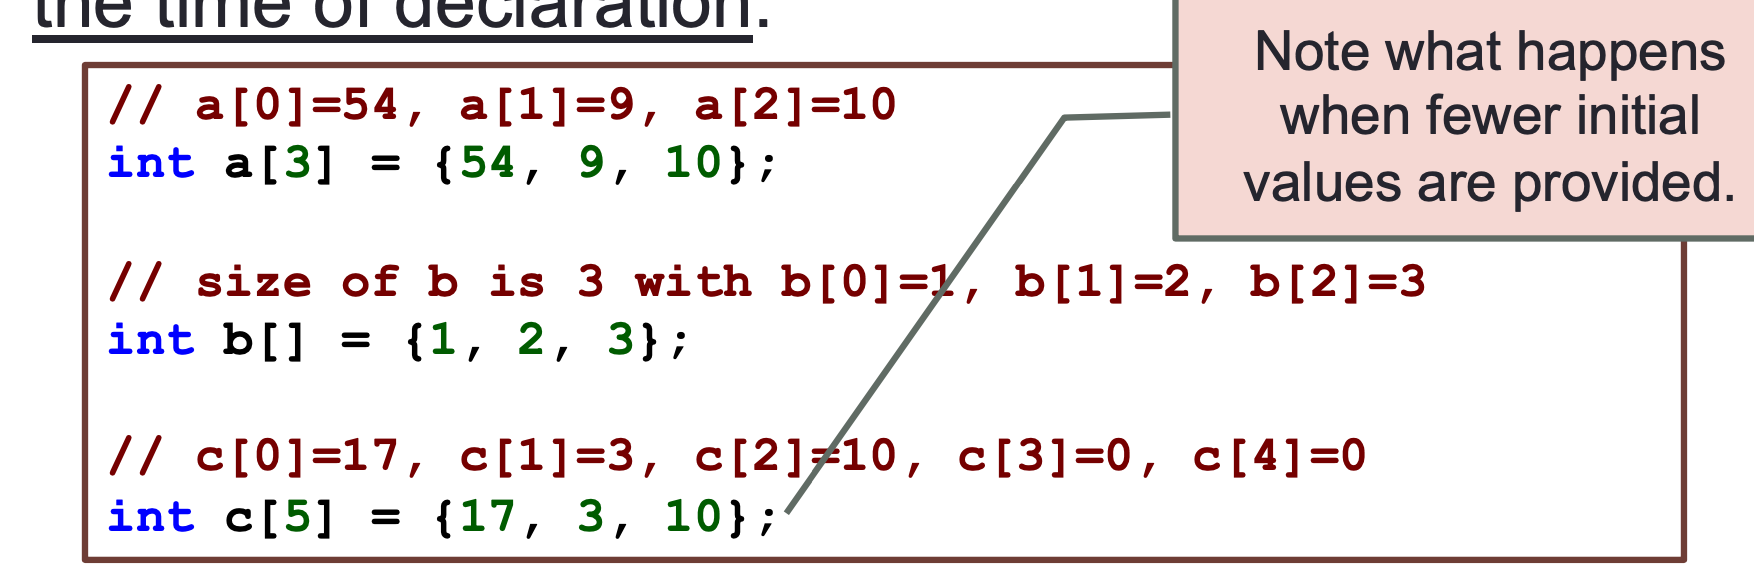
\includegraphics[scale=0.25]{./assets/array}\\
		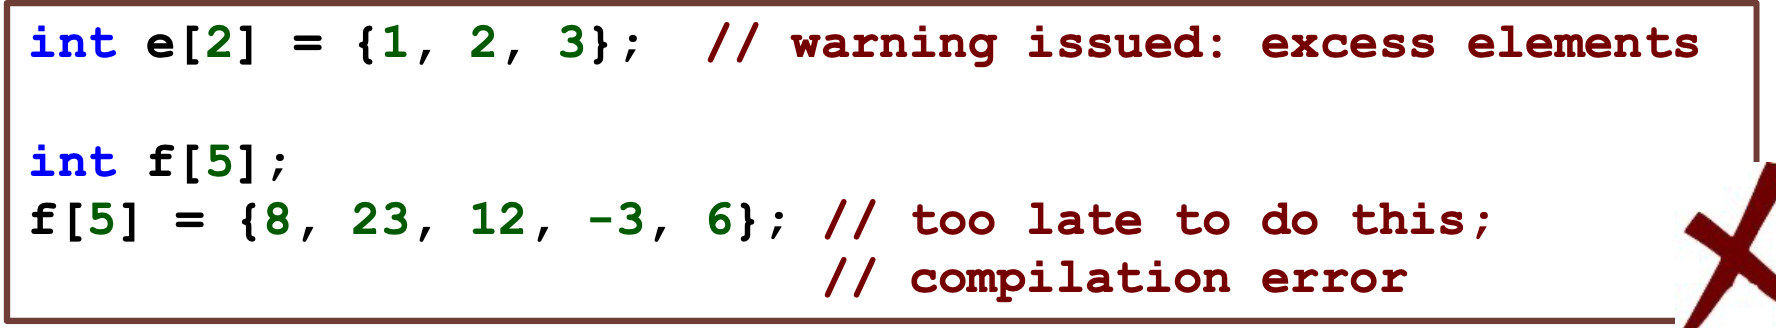
\includegraphics[scale=0.25]{./assets/array2}\\
		array name refers to the address of the first element \\
		eg. \texttt{int a[10]; // a = \&a[0]}\\
		
		\textbf{Array Assignment}\\
		Array name is a fixed pointer, it points to the first element in the array and cannot be altered
		\begin{verbatim}
			int source[10] = { 10, 20, 30, 40, 50 };
			int dest[10];
			dest = source; //illegal
		\end{verbatim}
		Instead use a loop to loop through elements and copy them over, or use \texttt{memcpy()} in $<$string.h$>$ library\\
		
		\textbf{Array params in functions}\\
		Function prototype: \texttt{int sumArray(int [], int);}\\
		Function Definition: 
		\begin{verbatim}
			int sumArray(int arr[], int size) { ... }
			int sumArray(int arr[8], int size) { ... }
		\end{verbatim}
		- 8 is ignored by the compiler because array parameters are passed in as pointers, must pass in size as a separate parameter\\
		- Therefore, alternative function prototype: \texttt{int sumarray(int *, size)} and alternative function definition: \texttt{ int sumArray(int *arr, int size) \{...\} }\\
		- This also means that any function can modify an array it receives\\
		
		\textbf{Strings}\\
		- Array of chars $\neq$ string, need to append null character\\
		- String is an array of chars terminated by a null character, (\textbackslash 0, ascii value 0)\\
		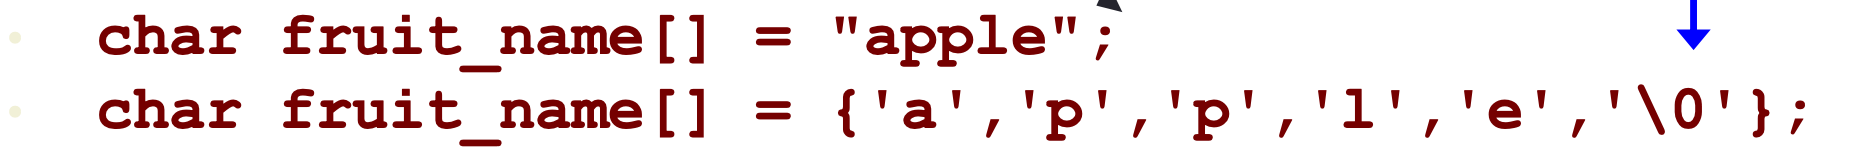
\includegraphics[scale=0.25]{./assets/stringInitialise}\\
		
		\textbf{String IO}\\
		Input:\\
		1. \texttt{fgets(str, size, stdin) // reads size - 1 char, or until (including) newline}\\
		2. \texttt{scanf("\%s", str); // reads until whitespace}\\  
		- Don't use \texttt{gets()}, can result in buffer overflow\\
		- \texttt{fgets()} can reads in newline character if there is enough space, need to replace it with null character
		\begin{verbatim}
			fgets(str, size, stdin);
			len = strlen(str);
			if (str[len - 1] == '\n') {
			    str[len - 1] = '\0';
			}
		\end{verbatim}
			
 		Output:\\
		1. \texttt{puts(str); // terminates with new line}\\
		2. \texttt{printf("\%s\textbackslash n", str); }\\
		
		\textbf{String Functions}\\
		1. \texttt{strlen(s)}, returns number of chars in s\\
		2. \texttt{strcmp(s1, s2)}, compares ASCII values of chars in s1 and s2, return negative int if s1 $<$ s2 and positive if s1 $>$ s2, 0 if same\\
		3. \texttt{strncmp(s1, s2, n)}, compares first n characters of s1 and s2\\
		4. \texttt{strcpy(s1, s2)}, copies s2 into s1, must use this because cannot assign, unless at declaration. If s2 too long can cause buffer overflow\\
		5. \texttt{strncpy(s1, s2, n)}, copies first n chars from s2 to s1\\
		All the functions use null character, without it could result in illegal access of memory\\
		
		\textbf{Structures}\\
		Structures allow grouping of members of different types\\
		A group can be a member of another group\\
		Groups are also called structure types\\
		
		Struct Definition:
		\begin{verbatim}
			typedef struct {
			    int acctNum;
			    float balance;
			} account_t;
		\end{verbatim}
		- Remember the ; at the end!\\
		- Types must be defined before declaring variables of that type\\
		- No memory is allocated to a type\\
		- Put struct definitions before function prototypes but after preprocessor directives\\
		
		\textbf{Accessing members of a structure variable}\\
		- Use the dot (.) operator\\
		eg:
		\begin{verbatim}
			result_t result;
			result.stuNum = 123456;
			result.score = 62.0;
			result.grade = 'D';
			
			card_t card = { 123456, {30, 6} };
			card.expiryDate.year = 2021;
		\end{verbatim}
		
		\textbf{Reading a Structure member}\\
		Structure members are read in individually
		\begin{verbatim}
			result_t result;
			printf("Enter student number, score and grade: ");
			scanf("%d %f %c", &result.stuNum, &result.score, &result.grade);
		\end{verbatim}
		Unlike arrays, can do assignment with structures, eg if result has already been initialised, result.stuNum = result1.stuNum is valid\\
		
		\textbf{Stuctures and Functions}\\
		
		Returning structure from function\\
		Can return a struct as you would for other types\\
		
		Structures as parameters\\
		- Uses pass-by-value, entire structure is copied over\\
		- To modify a structure's content, need to pass address of structure to function, using \& operator\\
		- Therefore to access members need to use (*player).name, for example. 
		- \highlight{Note} that dot operator (.) has higher precedence than indirection operator (*), therefore the () are needed\\
		- (*ptr\_name).member can be rewritten as ptr\_name--$>$member\\
		
		{\normalsize\textbf{MIPS}}\\
		\textbf{Overview}\\
		Mips uses Load-Store architecture, ie. both instructions and data are stored in memory\\
		- Limit memory operations\\
		- Rely on registers (mips has 32) for storage during execution\\
		\highlight{Note} that Registers have no data type!!\\
		
		\textbf{Arithmetic Operations}\\
		Addition and Subtraction\\
		eg. texttt{add \$s0, \$s1, \$s2}, adds \$s1 and \$s2 and stores in \$s0\\
		eg. texttt{sub \$s0, \$s1, \$s2}, subtracts \$s2 from \$s1 and stores in \$s0\\		
		
		Immediate operations\\
		Immediate values are constants, 16-bit, source2 is a constant instead\\
		Values ranges from $[-2^{15}$ to $2^{15}-1]$, 16-bit 2s comp\\
		
		Register Zero\\
		\$0 always has a value of 0\\
		Can be used to assign values eg \texttt{f = g}, by writing \texttt{add \$s0, \$s1, \$zero}, f in \$s0, g in \$s1\\
		
		\textbf{Logical Operators}\\
		View Registers as 32 raw bits instead of a number\\
		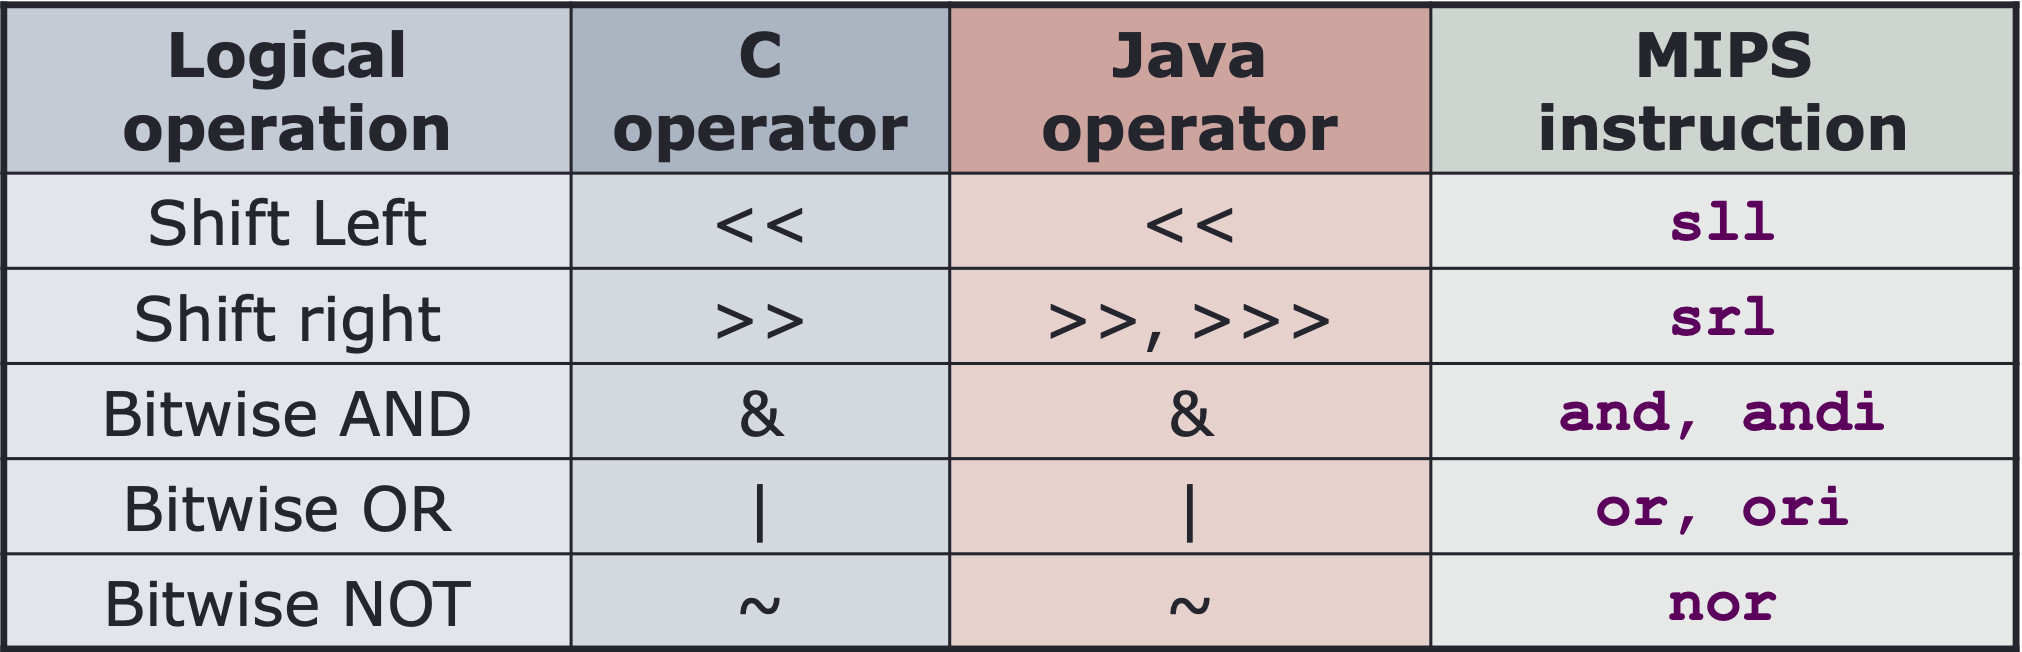
\includegraphics[scale=0.25]{./assets/logicalOperators}\\
		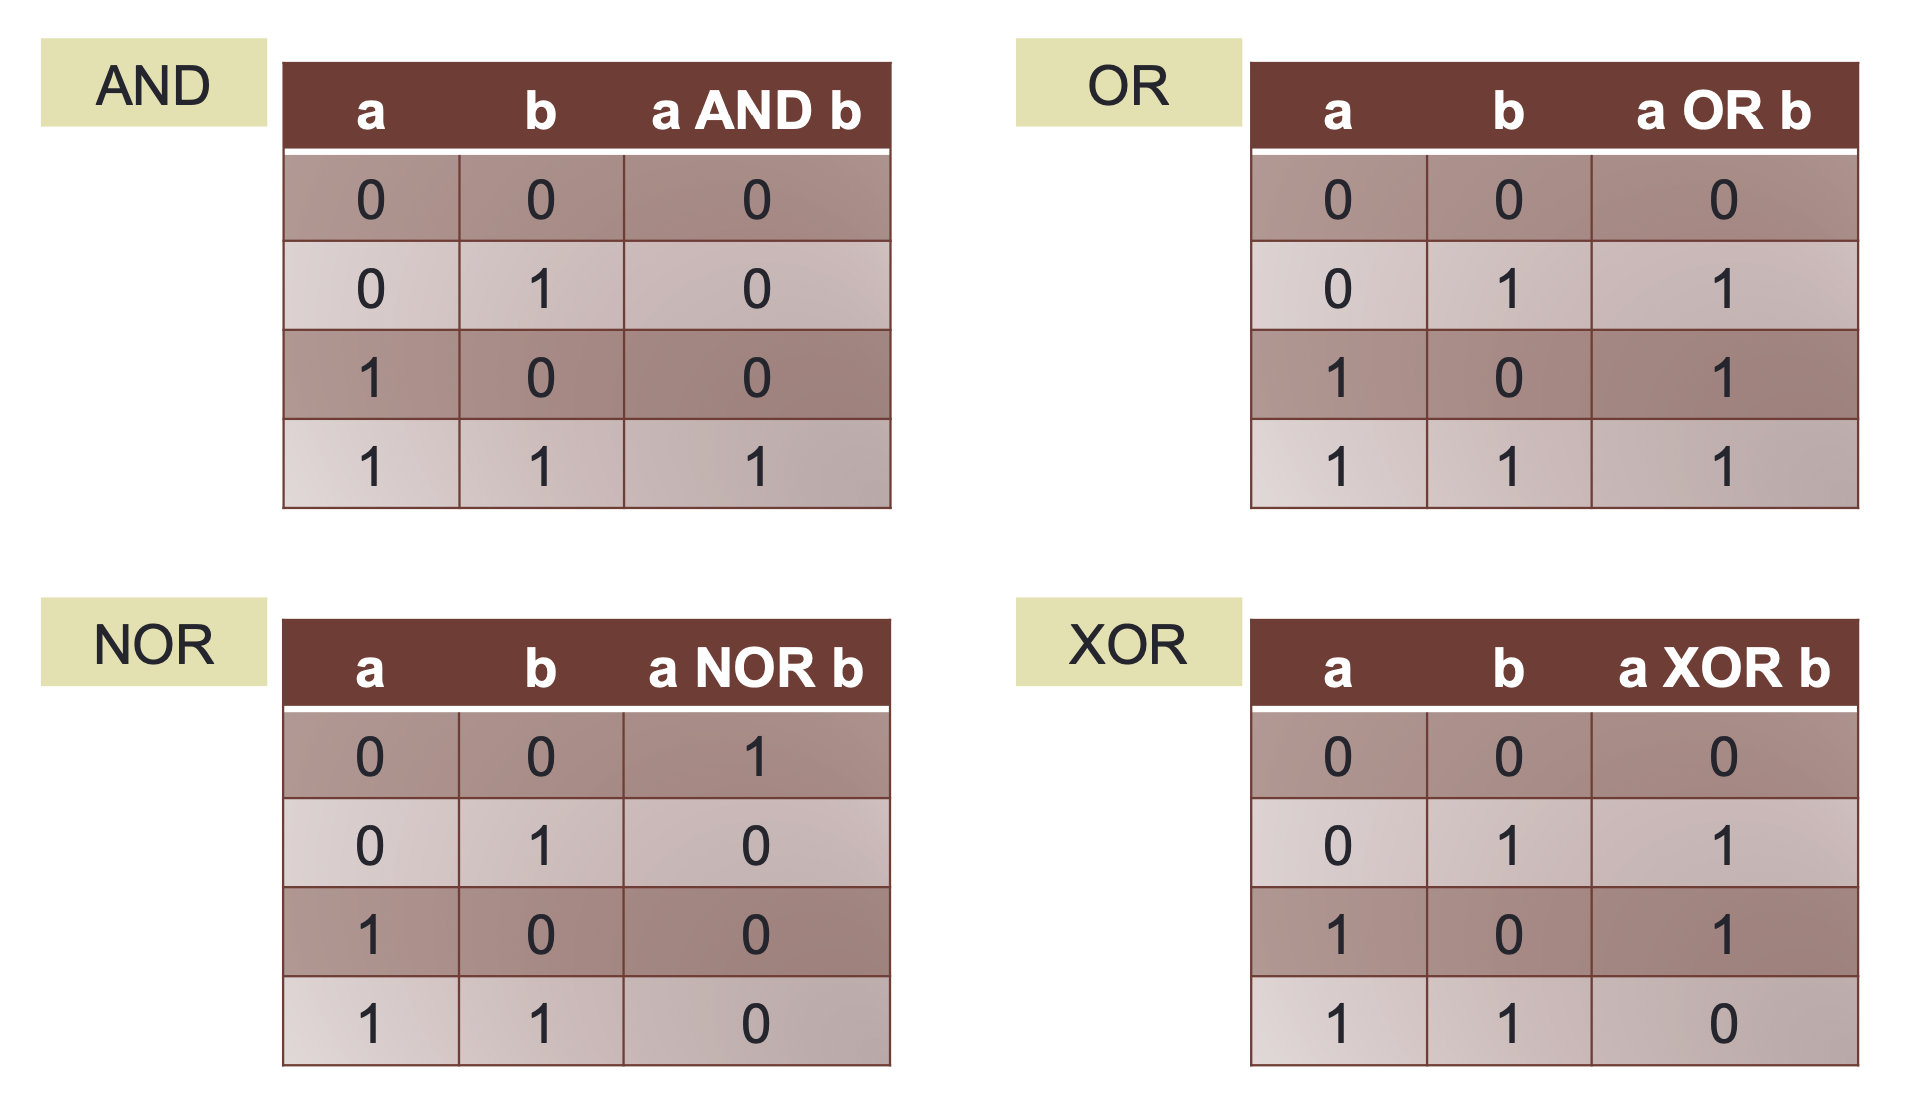
\includegraphics[scale=.25]{./assets/truthTables}\\
		
		Shift Left\\
		- sll (shift left logical): Move all bits in a word to the left by a number of positions; fill the emptied positions with zeroes.\\
		- has the effect of multiplying number by $2^n$, where n is the number in the immediate field\\
		
		Shift Right\\
		- srl (shift right logical): Move all bits in a word to the right by a number of positions; fills the emptied positions with zeroes.\\
		- divide number by $2^n$\\
		
		AND\\
		- $a \wedge 0 \implies 0$\\
		- $a \wedge 1 \implies a$\\
		- use above two properties for masking, set positions to be ignored to $0$, set positions of interest to $1$\\
		OR\\
		- $a \lor 0  \implies a$\\
		- $a \lor 1 \implies 1$\\
		- use above two properties for setting buts, set position to be set to 1\\
		
		NOR\\
		- Can be used to implement NOT instruction\\
		- NOR with 0\\		
		
		XOR\\
		- Can also be used to implement NOT instruction\\
		- XOR with 1\\
		- Has XORI instruction but no NORI, to keep instruction set small\\
		
		Large constant\\
		- How to load a 32 bit constant into a register\\
		- use \texttt{lui} instruction to set upper 16 bits (lower 16 bits would be set to 0)\\
		- then use \texttt{ori} instruction to set lower bits, (16 bit immediate would be 0-extended to 32-bit)\\
		\highlight{Note} that logical operators 0 extend immediates to 32 bits whereas arithmetic operations sign-extend(extend first bit)\\

		\textbf{Memory Instruction}\\
		Load Word\\
		- eg \texttt{lw \$t0, 4(\$s0)}
		- address = value of \texttt{\$s0} + $4$, eg $8000$ stored in \texttt{\$s0}, then address = $8004$\\
		- Memory word at \texttt{Mem[8004]} loaded into \texttt{\$t0}, ie \texttt{Mem[8004] - Mem[8007]}\\
		Store Word\\
		- eg \texttt{sw \$t0, 12(\$s0)}
		- address = value of \texttt{\$s0} + $12$, eg $8000$ stored in \texttt{\$s0}, then address = $8012$\\
		- Content of \texttt{\$t0} stored into the word at \texttt{Mem[8012], ie, 8012 - 8015}\\
		
		- \highlight{Note} that offset must be a multiple of 4 (because word is 4 bytes in mips)\\
		- MIPS does not allow unaligned load and stores with lw and sw, need to use pseudo-instructions ulw and usw\\
		- Other load-store instructions include load byte \texttt{(lb)} and store byte \texttt{(sb)}, used for chars and char arrays, for these instructions, offset no need multiple of 4\\
		  
		\textbf{Decisions}\\
		1. Conditional (branching)\\
		2. Unconditional (jump)\\
		
		\textbf{Branching}\\
		BEQ, branch on equal\\
		- eg \texttt{beq \$r1, \$r2, label}\\
		- go to the statement labeled \texttt{label} if value in \$r1 is equal to value in \$r2\\
		BNE, branch not equal\\
		- eg \texttt{bne \$r1, \$r2, label}\\
		- go to the statement labeled \texttt{label} if values aren't equal\\
		
		\textbf{Jump}\\
		- processor always follows the branch\\
		- eg \texttt{j label}\\
		
		\highlight{Note} that label is an "anchor" in code. Labels are not instructions\\
		- Later on labels will be converted to numbers, ie PC relative addressing for branch and truncated adress for jump\\
		Common technique: when there is only one branch, ie if with no else, then invert the conditional for more succint code\\
		
		\textbf{Inequalities}\\
		For branch on less than or branch on greater than, use slt\\
		- slt (slti): set on less than eg \texttt{slt \$t0, \$s1, \$s2}, sets \$t0 to 1 if \$s1 $<$ \$s2 or 0 otherwise\\
		- use slt with beq or bne to achieve blt or bgt (reverse \$s1 and \$s2 in slt)
		\begin{verbatim}
			blt $s1, $s2, L
			
			slt $t0, $s1, $s2 # these two instructions equivalent to above
			bne $t0, $zero, L
		\end{verbatim}
		\textbf{Arrays and loops}\\
		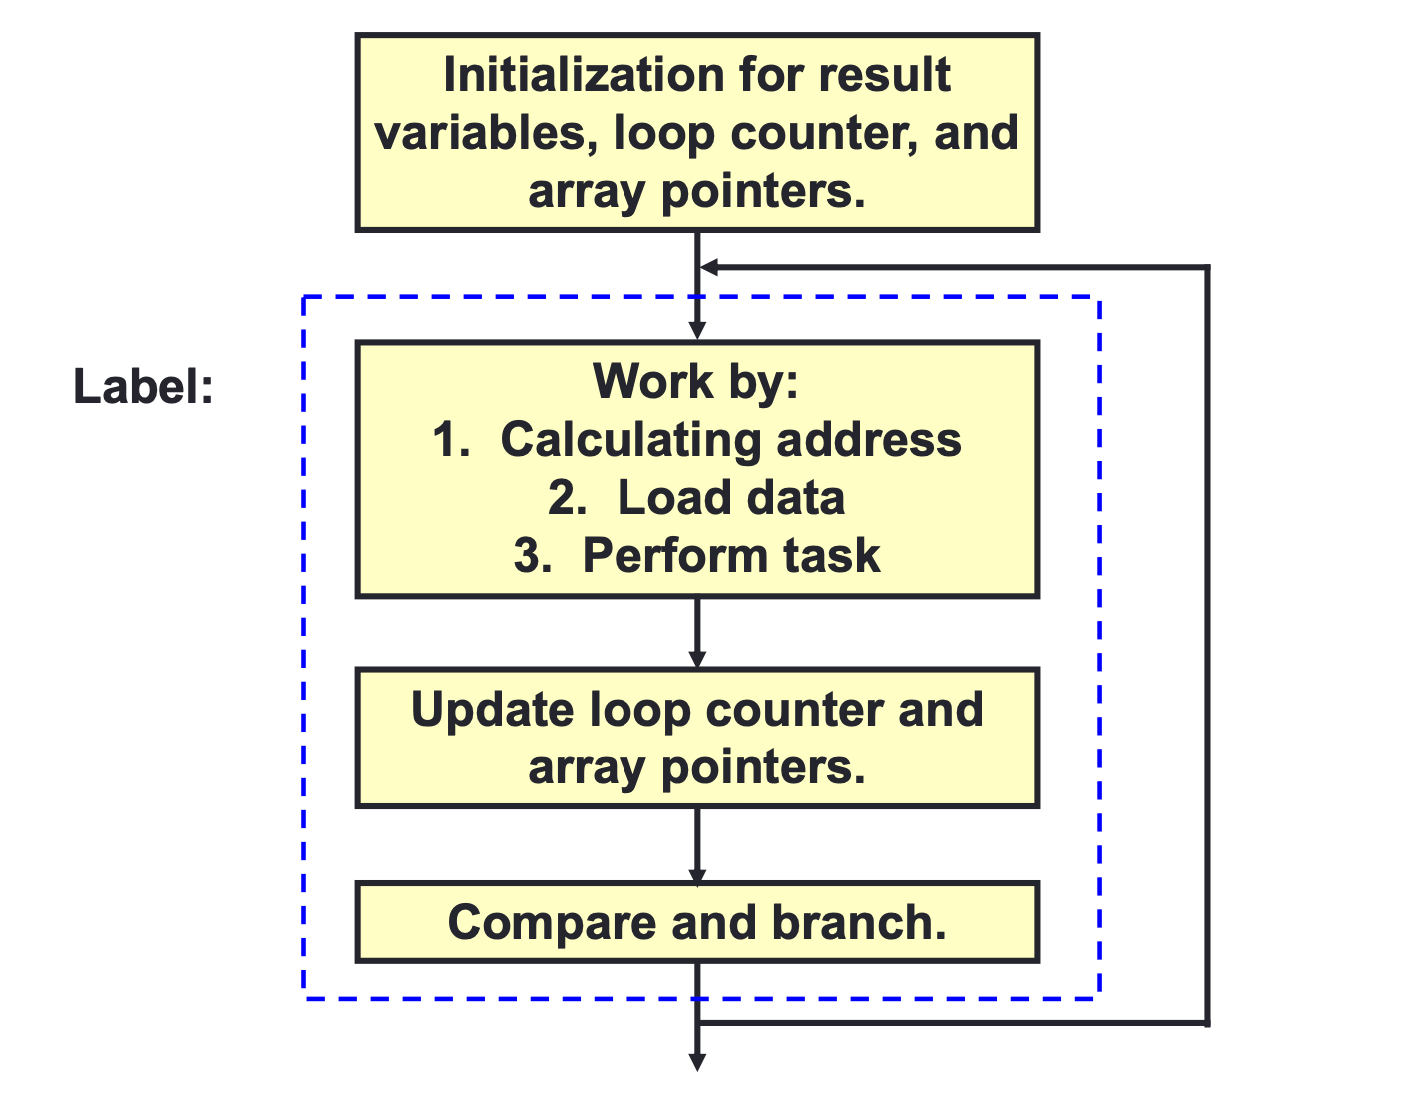
\includegraphics[scale=0.3]{./assets/arrayFlowchart}\\
		Can use pointers instead of index to make code shorter. \\
		- index need to increment, shift left twice (if 4 bytes like int) unless array of chars, then add to base address\\
		- using pointers, set pointer to base address, increment by 4 each time (if int/ float etc), or increment by 1 if char array\\
		
		\textbf{Encoding Instructions}\\
		Constraints are to encode all instructions in 32 bits, and make them as regular as possible\\
		1. R-format (Register format: \texttt{op \$r1, \$r2, \$r3})\\
		2. I-format (Immediate format: \texttt{op \$r1, \$r2, Immd})\\
		3. J-format (Jump format: \texttt{op Immd})\\
		
		\textbf{Instruction Address}\\
		- Instructions stored in memory\\
		- Instructions are 32-bits long\\
		- Instructions are word-aligned\\
		Program Counter (PC) is a special register that keeps the address of the instruction being executed by processor\\
		
		\textbf{Branch Instruction Encoding}\\
		Immediate is only 16-bits, addresses are 32 bits. Immediate is not long enough\\
		- Specify target address \textbf{relative to PC}\\
		- Since instructions are word aligned, can treat the immediate as number of \textit{words} away from PC\\
		- Can branch up to $2^{15}$ words away from PC, $2^{17}$ bytes\\
		Branch Calculation:\\
		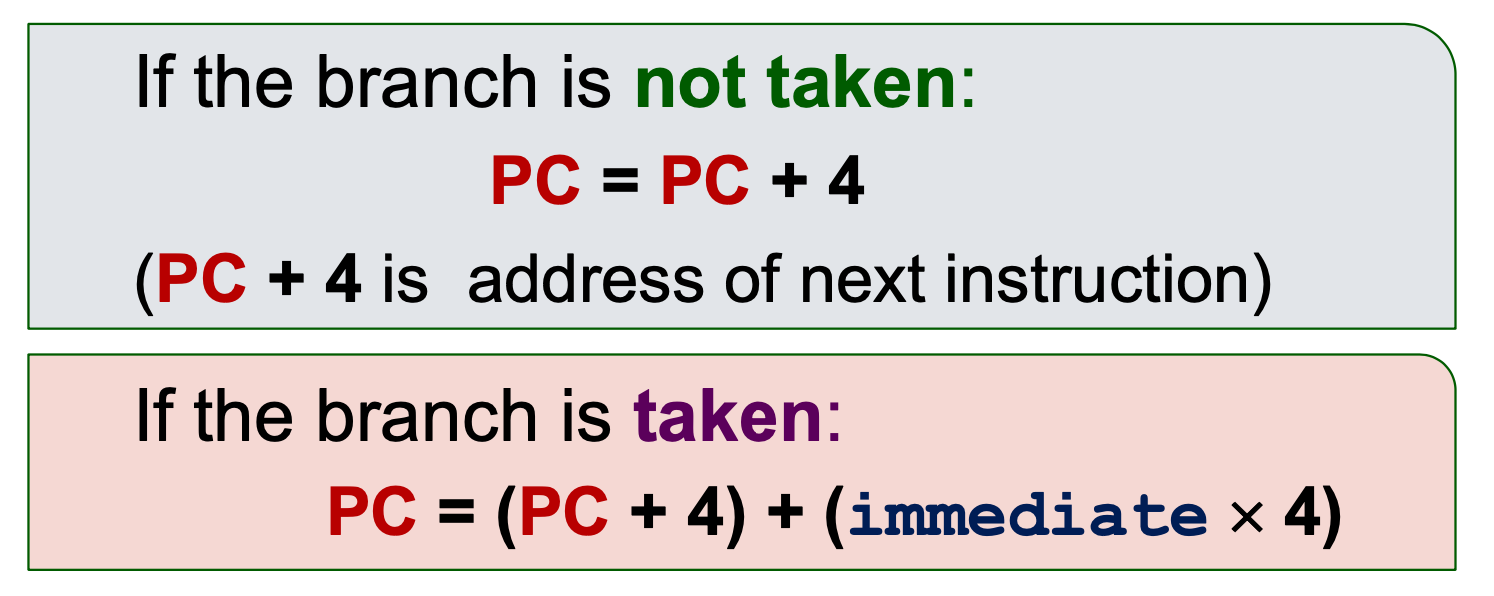
\includegraphics[scale=.25]{./assets/branchCalculation}\\
		\highlight{Note}: immd field specifies number of words to jumps, which is the \textbf{same} as the number of instructions to skip over\\
		
		\textbf{J-format}\\
		For jumps, can jump anywhere in memory, not small jumps so cannot use PC-relative addressing\\
		Want to specify a 32-bit address to jump to, but cannot due to 6-bit opcode\\
		Getting the address:\\
		1. Start with 26-bits\\
		2. Instructions are word aligned, so last two bits are always 00, can omit (like branching), now have 28-bit\\
		3. Choose \textbf{4 most significant bits from PC+4}, cannot jump to anywhere in memory but should be sufficient. Max jump range: 256MB boundary\\
		
		\textbf{Summary}\\
		- Branches and load/store are both I-format instructions, but branch use \textbf{PC-relative addressing} while load/store uses \textbf{base addressing}\\
		- Jumps use \textbf{pseudo-direct addressing}\\
		- shifts use R-format, but other immediate instructions use I-format\\
		
		{\normalsize\textbf{Instruction Set Architecture}}\\	
		\textbf{5 concepts of ISA design}\\
		1. Data Storage\\
		2. Memory Addressing Modes\\
		3. Operations in Instruction Set\\
		4. Instruction Formats\\
		5. Encoding the Instruction Set\\
		
		\textbf{1. Data Storage}\\
		\includegraphics[scale=.2]{./assets/dataStorage}\\
		
		\textbf{2. Memory Addressing Mode}\\
		- Given $k$ bit address, address space is of size $2^k$\\
		- Each memory transfer consists of one word of $n$ bits\\
		Procesor contains:\\
		- Memory Address Register (MAR): k-bit address bus between processor and memory (one direction cpu $\rightarrow$ mem)\\
		- Memory Data Register (MDR): n-bit data bus (bidirectional for read and write)\\
		- control lines: eg read/write control\\
		
		\textbf{Endianness}\\
		The relative ordering of the bytes in a multiple-byte word stored in memory\\
		- Big-endian: MSB stored in lowest address\\
		- Little-endian: LSB stored in lowest address\\
		Eg. For \texttt{0xDE AD BE EF}\\
		- Big-endian: \texttt{0: DE, 1: AD, 2: BE, 3: EF}\\
		- Little-endiand: \texttt{0: EF, 1: BE, 2: AD, 3: DE}\\
		\highlight{NOTE}: Ordering \textbf{within} bytes are not affected, only ordering \textbf{between} bytes\\
		
		\textbf{Addressing Modes}\\
		In MIPS, 3 addressing modes\\
		1. Register: Operands in register\\
		2. Immediate: Operand is specified in instruction directly\\
		3. Displacement: Operand is in memory with address calculated as Base + Offset (lw/sw)\\
		
		\textbf{4. Instruction Format}\\
		Instruction Length:\\
		- Variable length: More flexible (but complex) and compact instruction set, requires multi-step fetch and decode\\
		- Fixed length: Easier fetch and decode, simplify pipelining and parallelism, but instruction bits are scarce\\
		
		\textbf{5. Encoding the Instruction Set}\\
		Things to be decided:\\
		- No. of registers\\
		- No. of addressing modes\\
		- No. of operands in instruction\\
		Expanding Opcode scheme for fixed length instructions\\
		- Opcode has variable length for different instructions\\
		Eg. 16 bit fixed length instruction, 2 types of instructions, 1 operand and 2 operand, each operand takes 5 bits\\
		- Type A: 6-bit opcode, $2 *$5-bit operand\\
		- Type B: 11-bit opcode, $1*$5-bit operand\\
		To maximise no. of instructions: Give more 6-bit prefixes to type B\\
		To minimise no. of instructions: Give more opcodes to type A\\
		
		{\normalsize\textbf{Datapath}}\\
		\textbf{Instruction Execution Cycle}\\
		1. Instruction Fetch: Get instruction from mem (address is in PC)\\
		2. Instruction Decode and Fetch Operands: Find out operation, get operands\\
		3. ALU: Arithmetic and Logical operations\\
		4. Memory Access: Memory operation (load/store)\\
		5. Result Write: Write back result of operation to register if needed\\
		\highlight{NOTE}: can merge instruction decode and operand fetch because decode is simple for MIPS\\
		
		\textbf{1. Instruction Fetch}\\
		1. Use PC to fetch instruction from memory\\
		2. Increment PC by 4 to get address of next instruction (recall instructions are 32-bits long)\\
		Exception is when branch or jump\\
		- PC is read during first half of the clock period and is updated with PC+4 ad the \textbf{next rising clock edge}, this prevents reading and updating PC at the same time\\
		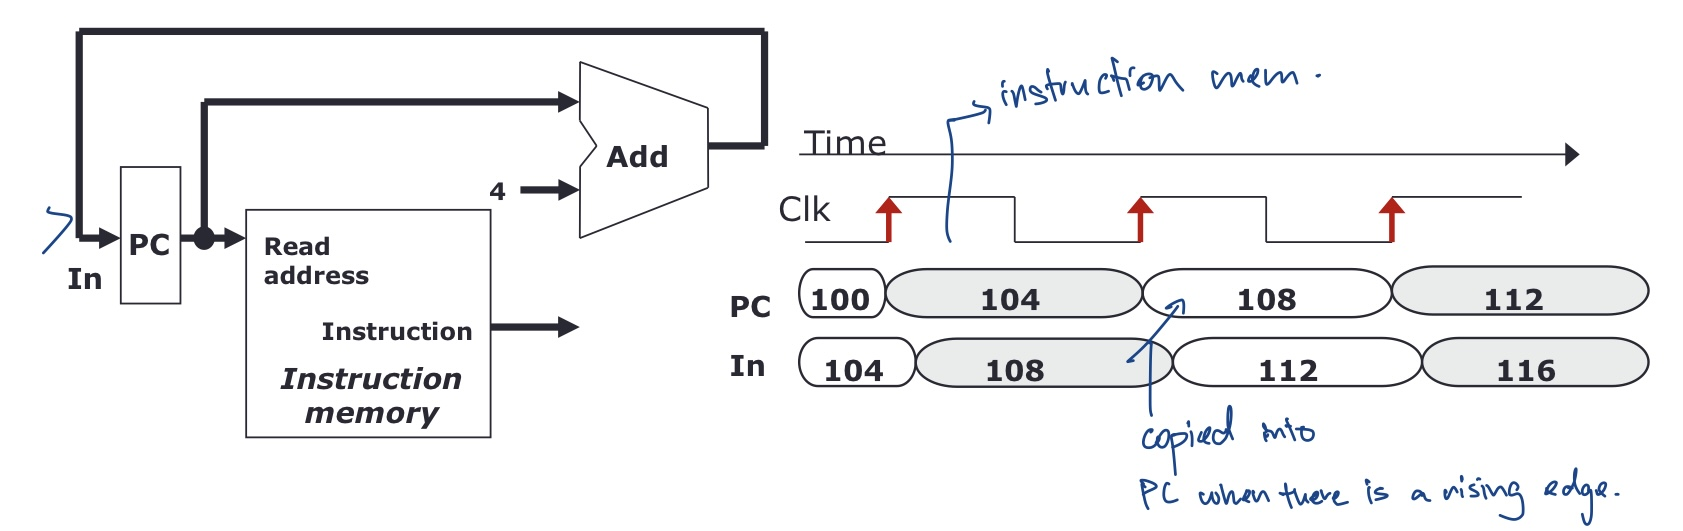
\includegraphics[scale=.15]{./assets/clock}\\
		
		\textbf{2. Instruction Decode}\\
		1. Read opcode to determine instruction type and field lengths\\
		2. read data from necessary registers\\
		- Register File: collection of 32 32-bit registers that can be read or written to\\
		- Each instruction reads at most 2 registers and writes to at most 1 register\\
		- \texttt{RegWrite} is the control signal to indicate writing fo register; 1 = write, 0 = no write\\
		- Need to use multiplexer with \texttt{RegDst} control signal to choose between \texttt{rt} and \texttt{immediate} for write register\\
		- Need to sign extend \texttt{immediate} to 32 bit and output to ALU\\
		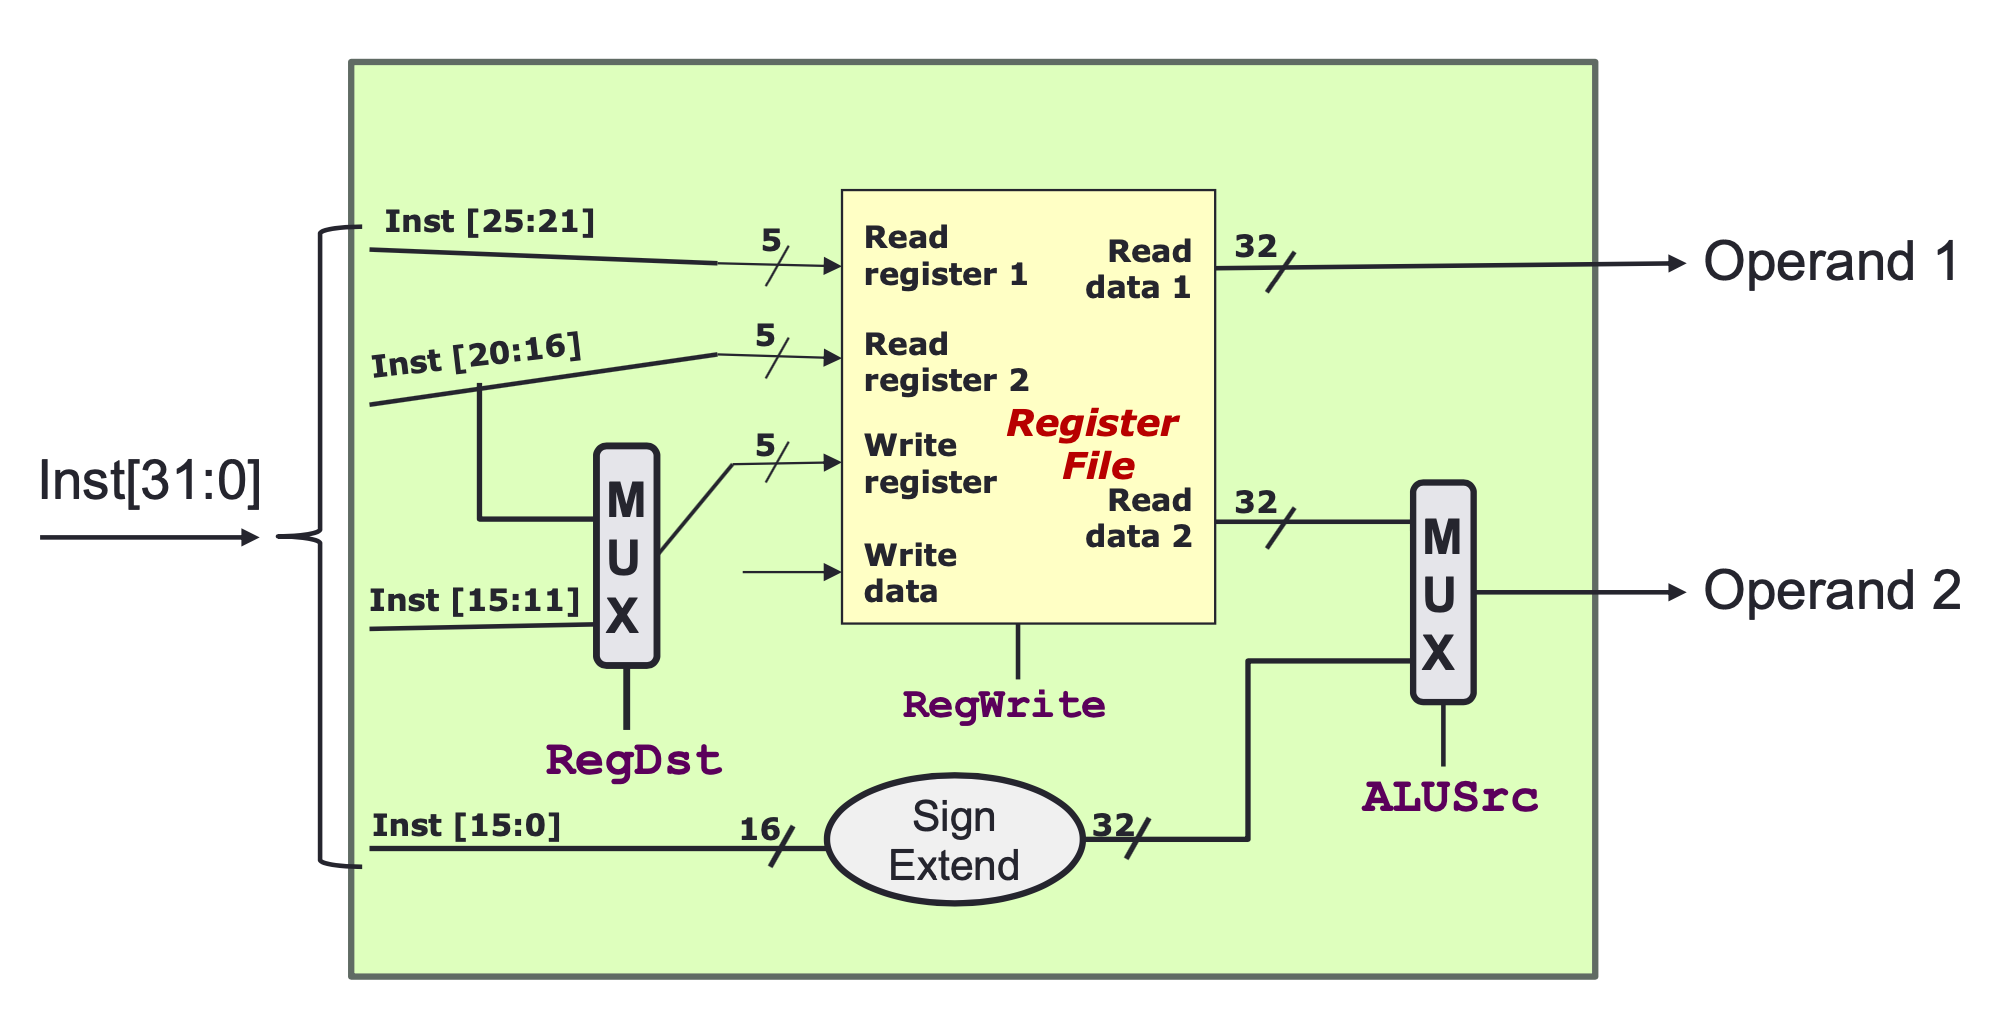
\includegraphics[scale=.2]{./assets/decodeStage}\\
		
		\textbf{3. ALU Stage aka EX stage}\\
		- takes in 2 32 bit numbers\\
		- outputs 32-bit result and 1 bit signal \texttt{isZero} for branching\\
		- 4-bit control signal called \texttt{ALUcontrol}\\
		
		Exception Branch instructions\\
		- need to perform 2 calculations: Branch outcome and target address\\
		- current circuit would be wrong because branching is I-format instruction (ALUSrc would send immediate to ALU instead of register)\\
		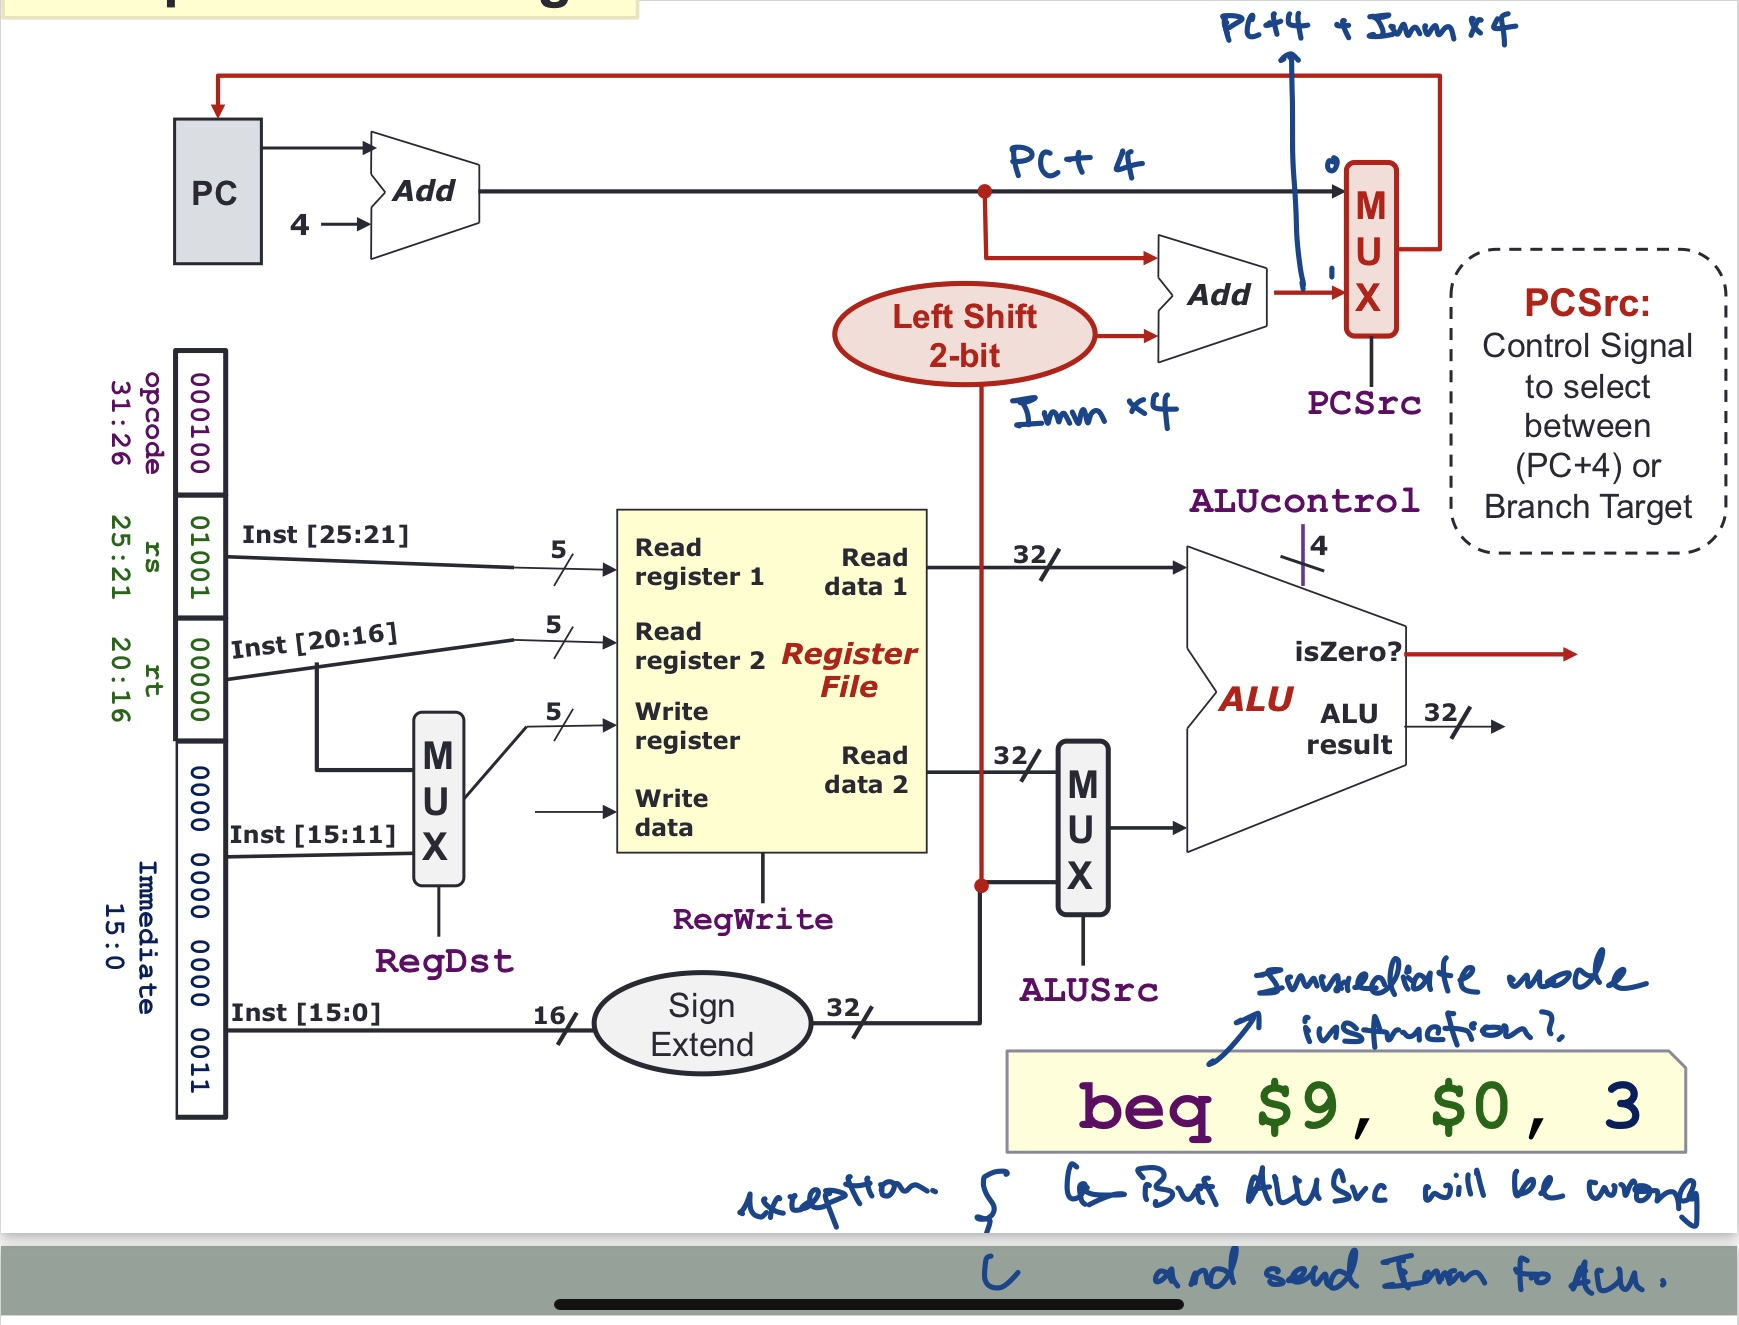
\includegraphics[scale=.15]{./assets/ALU}\\
		
		\textbf{4. Memory Stage}\\
		Only load and store instructions need to perform operations in this stage.\\
		- Use memory address calculated by ALU stage\\
		- Read or write to data memory\\
		All other instructions remain idle\\
		Data memory\\
		- Inputs: memory address, data to be written (Write Data) for store instructions\\
		- Output: Data read from memory for load instructions\\
		- Control: Read and write controls
		\begin{verbatim}
			R W
			1 1 undefined (should not have this case)
			0 1 write
			1 0 read
			0 0 nothing
		\end{verbatim} 
		For store instructions, need to connect RD2 (rt) to Write Data.\\
		Need to choose between output from Read Data and output from ALU stage\\
		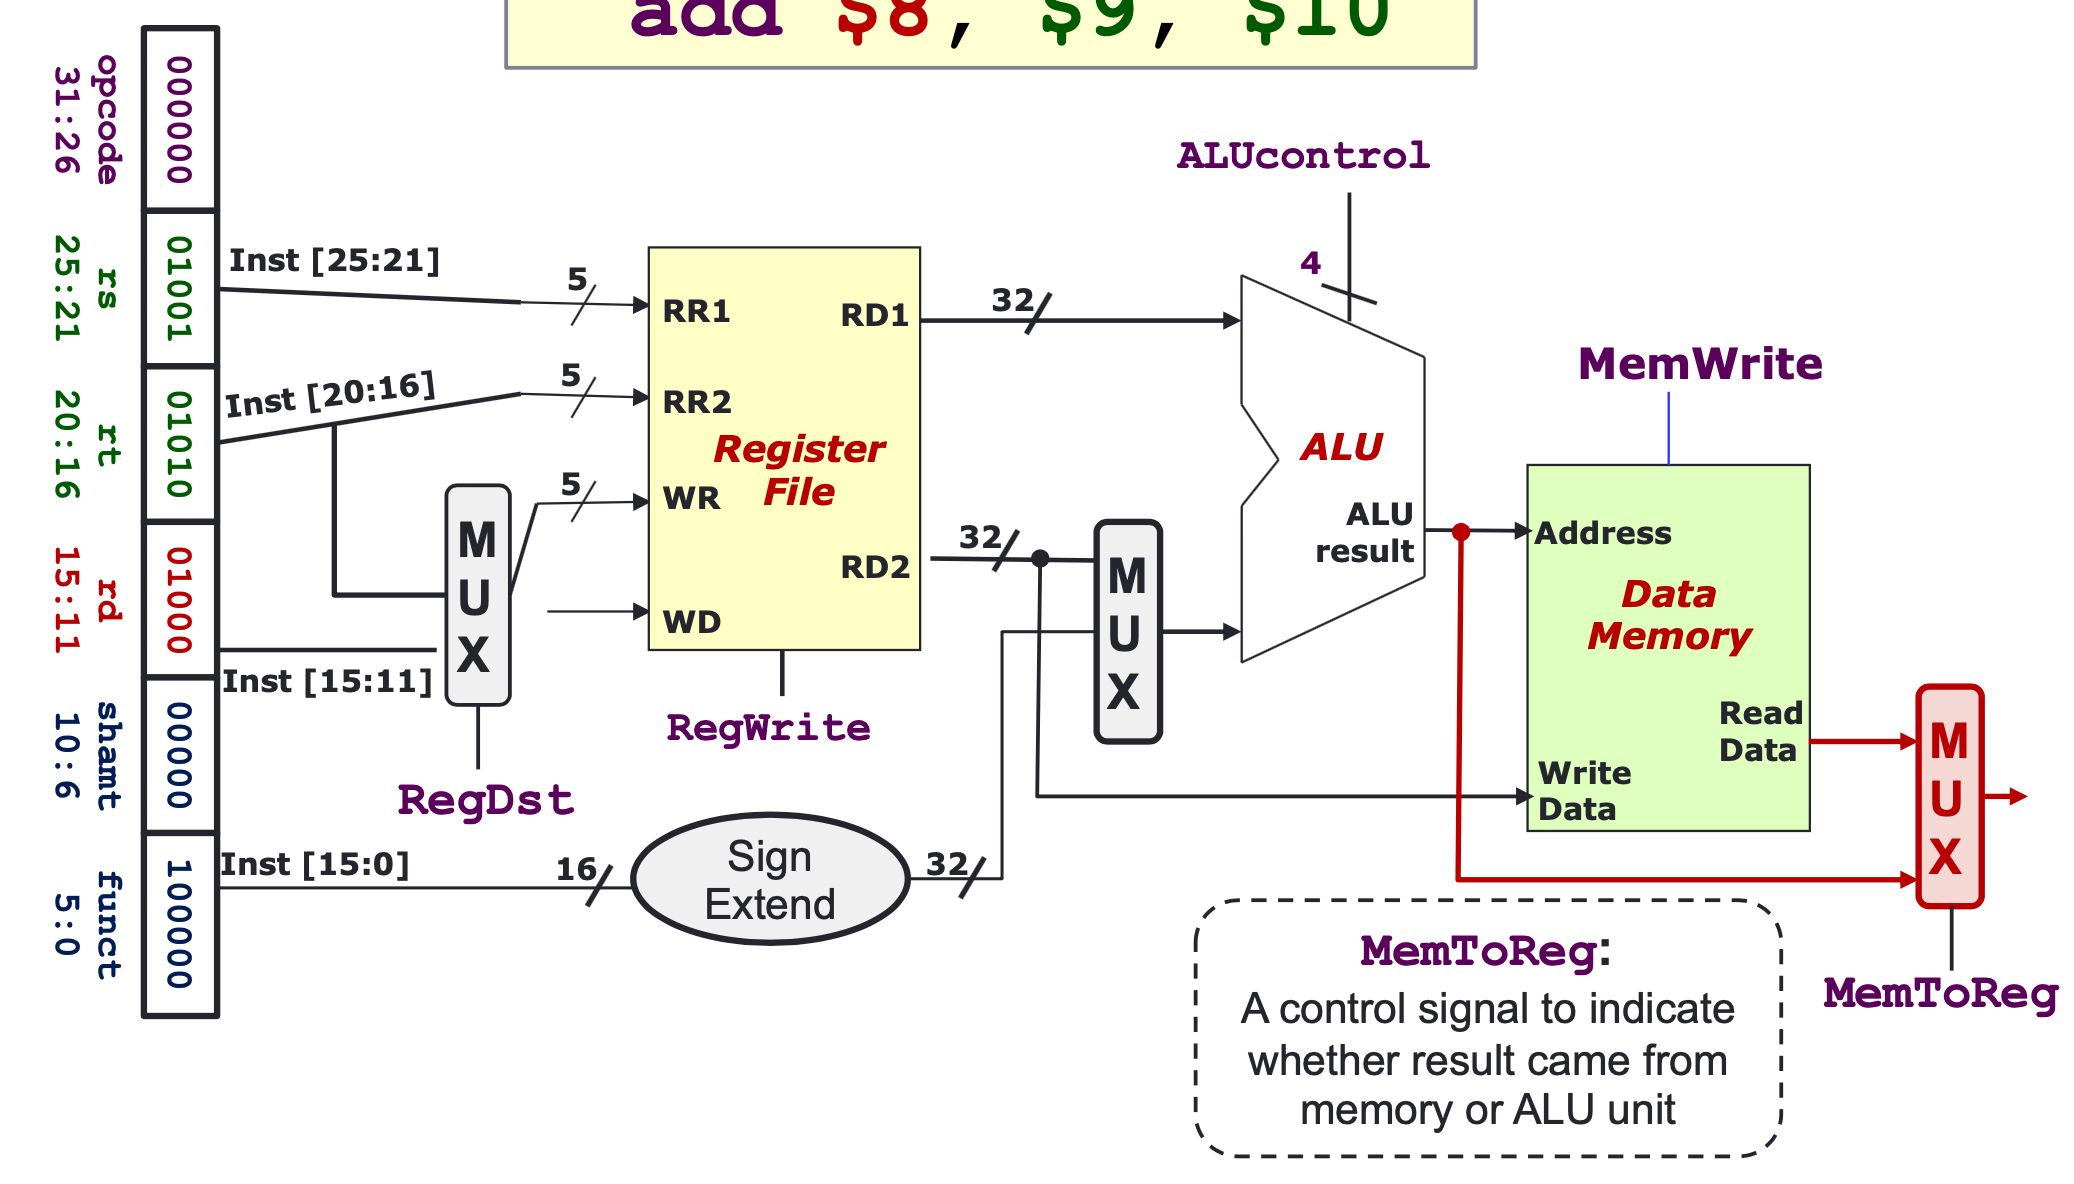
\includegraphics[scale=.25]{./assets/memStage}\\
		\highlight{NOTE}: MemToReg mux is mounted upside down ie. 1 is Read Data, 0 is ALU result\\
		 
		\textbf{5. Register Write Stage}\\
		Write to register (stores, arithmetics, loads, slt, etc)\\
		Just connect correct result to Register File Write Data input.\\
		- Control: RegWrite, 1 write 0 nothing\\
		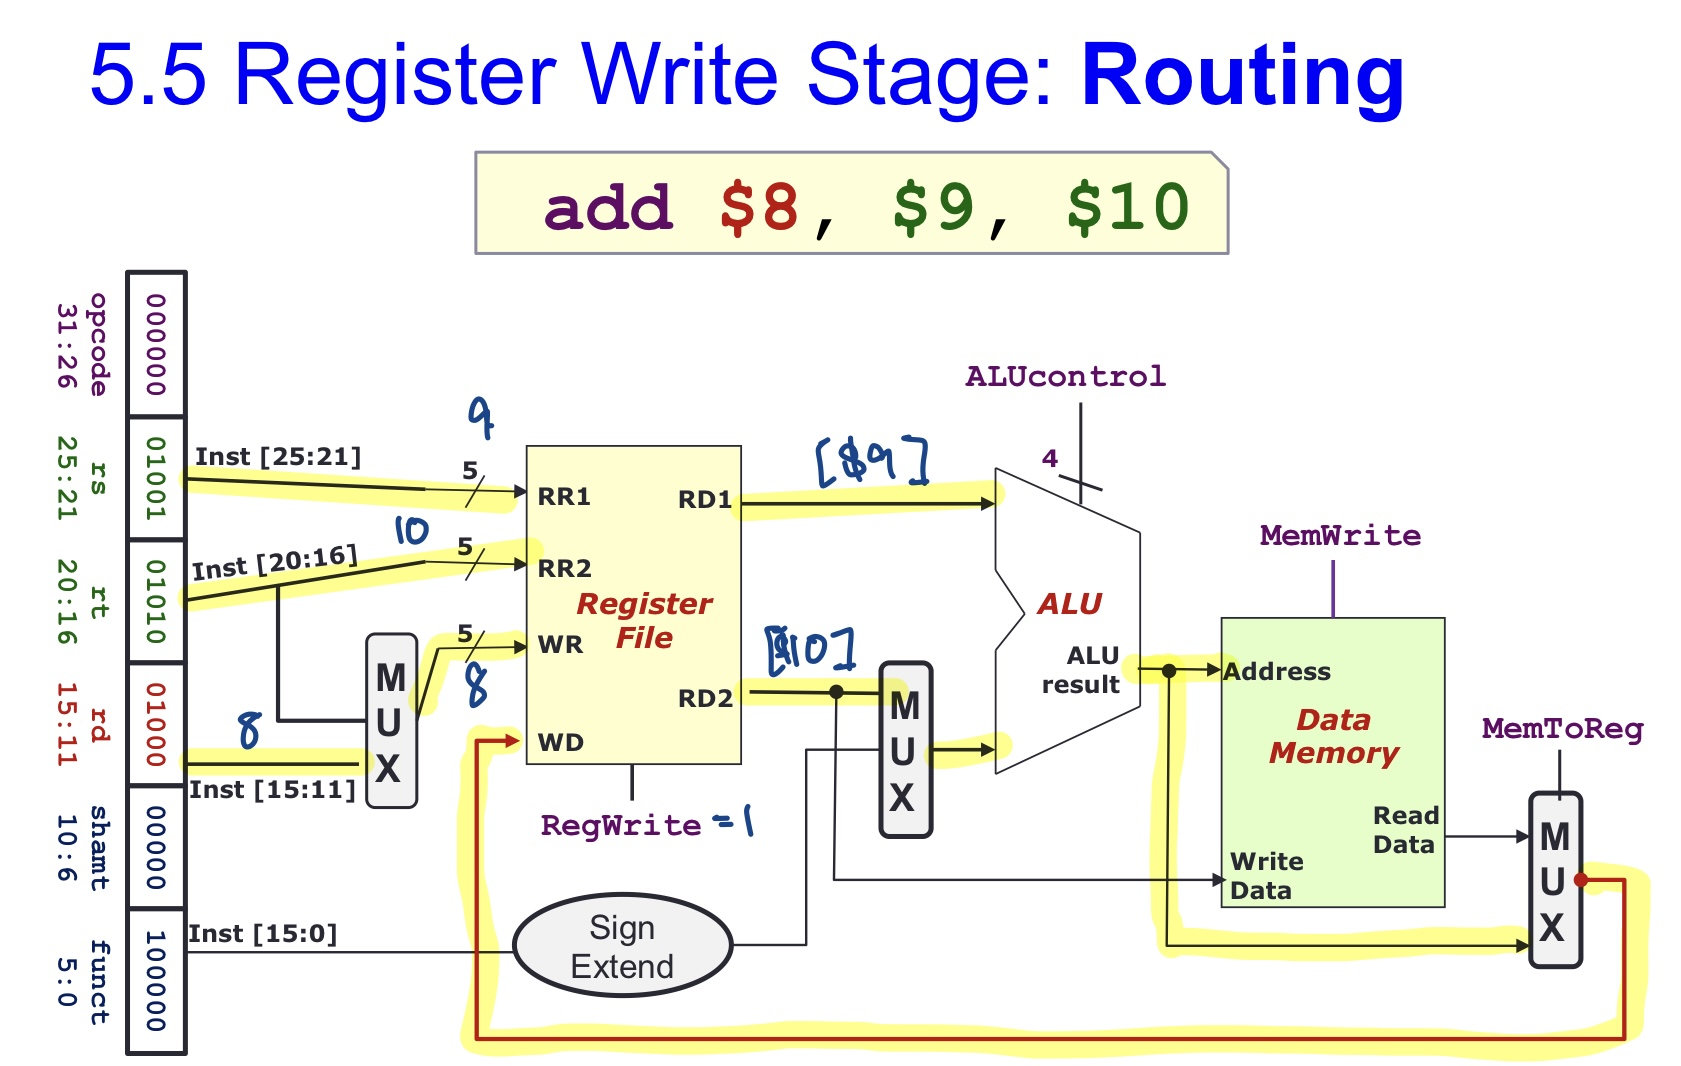
\includegraphics[scale=0.16]{./assets/regWrite}\\
		
		{\normalsize\textbf{Control}}\\
		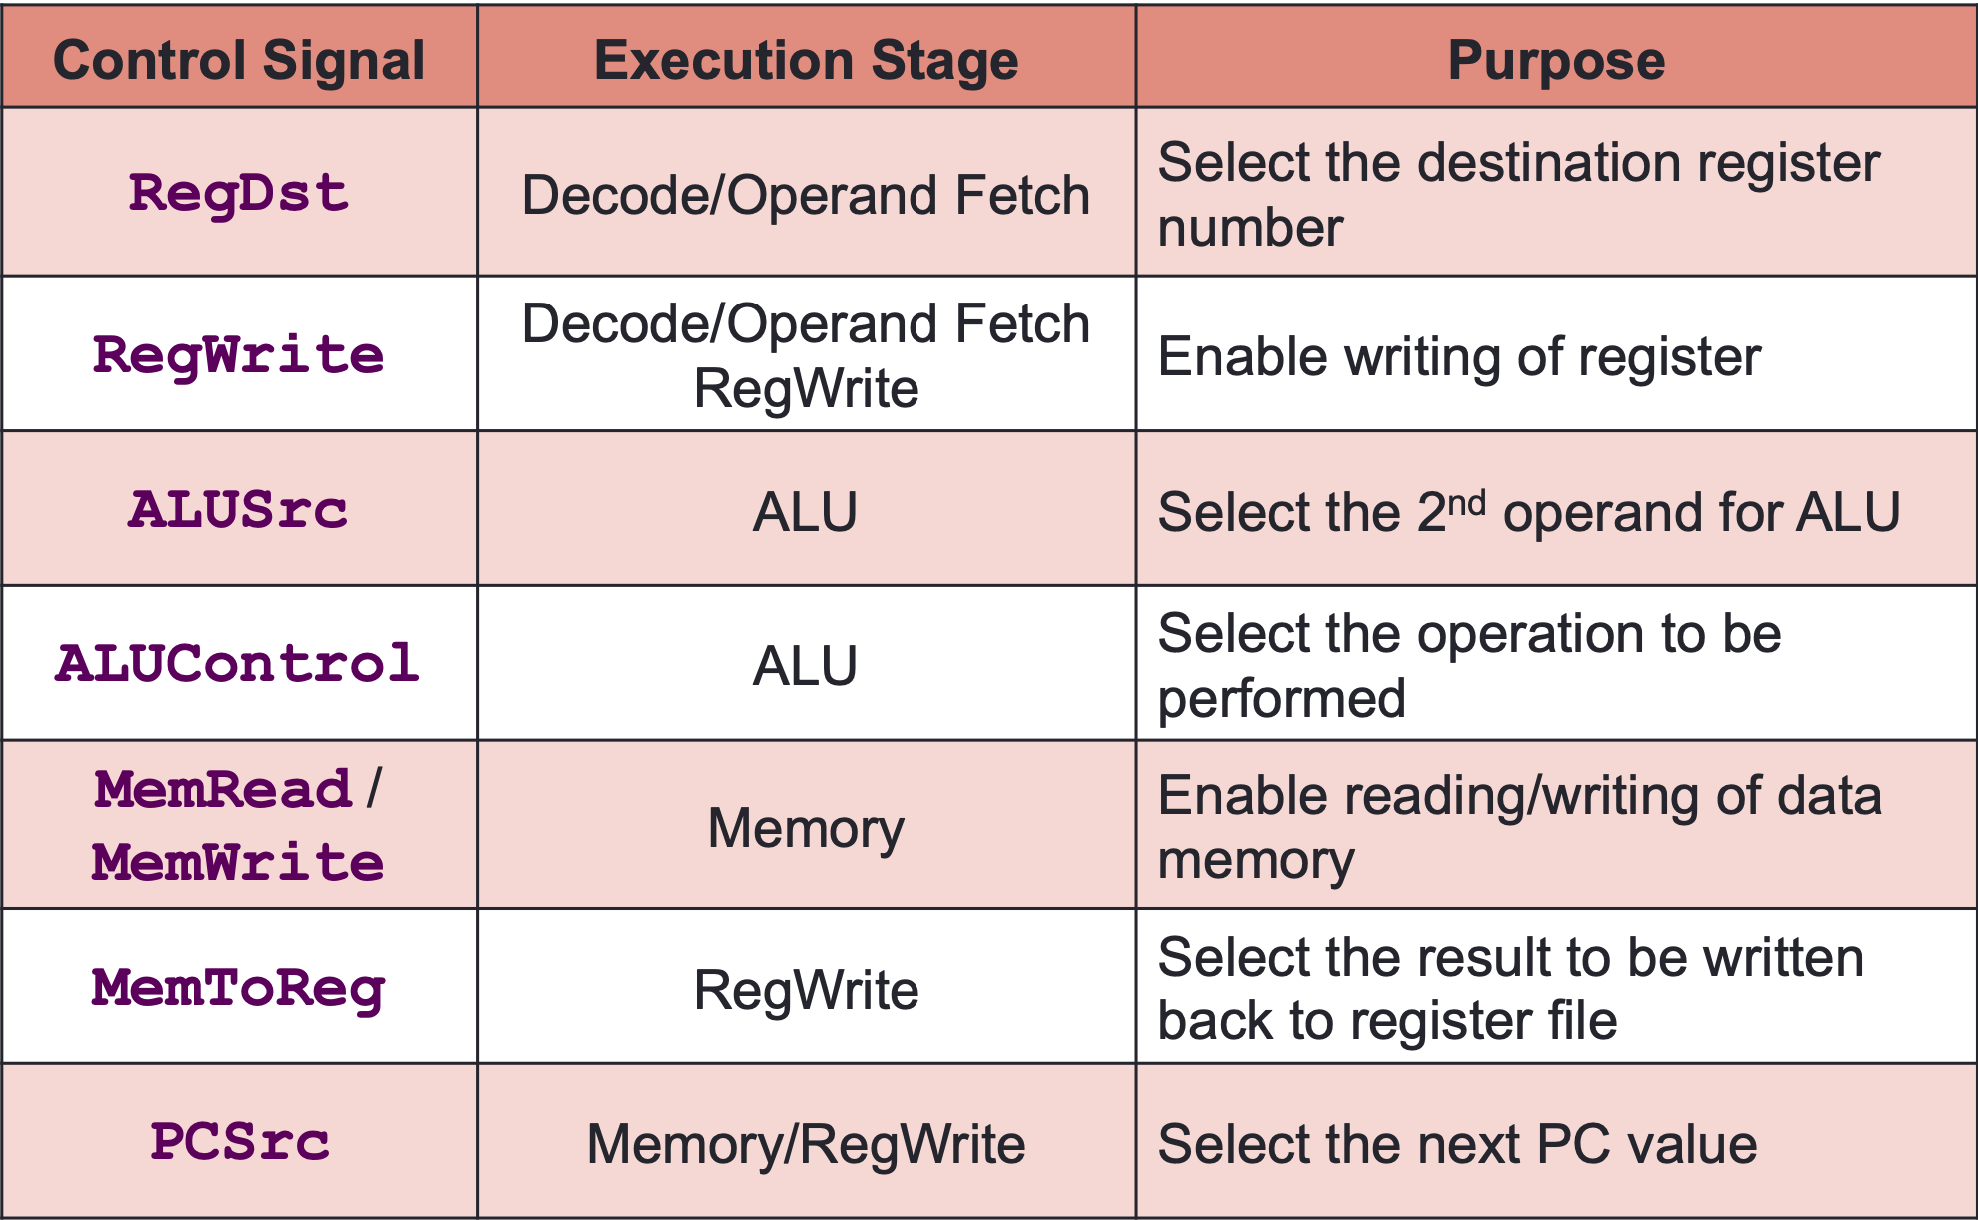
\includegraphics[scale=.26]{./assets/controlSignals}\\
		- Generate all of these signals using opcode (and funct, for R-type) using a combinational circuit\\
		
		\textbf{PCSrc}\\
		\highlight{Note} only need opcode (that it is a branch instruction) but also if the branch is taken (\texttt{isZero === 1}).\\
		- Therefore, need to combine the two signals using \texttt{AND} gate\\
		
		\textbf{ALUControl}\\
		All control signals other than ALUControl can be generated from opcode only (the signals are the same for all R-type), only ALUControl needs funct code (as opcode is 0 for all R-type)\\
		- only exception is shifts?\\
		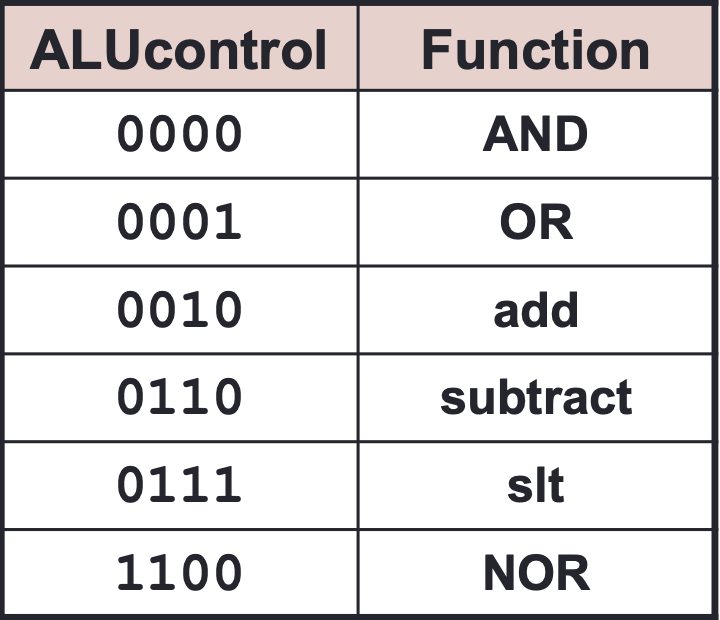
\includegraphics[scale=0.25]{./assets/ALUControl}\\
		\includegraphics[scale=0.25]{./assets/ALUCircuit}\\
		Picture shows 1 "slice" of 32-bit ALU. Can think of actual ALU as 32 slices back to back\\
		\highlight{NOTE}: \texttt{SUB} is implemented by inverting all bits in B, setting first $C_{in}$ to $1$
		
		\centerline{$A + B' + 1 = A +$ 2s comp of $B$}
		
		\textbf{Multilevel Decoding}\\
		- Use some of the input to reduce cases, then generate full output\\
		- Simplifies design process, reduce size of main controller, speedup circuit\\
		
		\textbf{Intermediate Signal: ALUop}\\
		- Use opcode to generate 2-bit \texttt{ALUop} signal
		\begin{verbatim}
			Instruction  |  ALUop  |  What
			lw/sw        |  00     |  ADD
			beq          |  01     |  SUB
			R-type       |  10     | depends on funct
		\end{verbatim}
		Use \texttt{ALUop} signal and \texttt{funct} field from R-type to generate 4-bit \texttt{ALUControl}\\
		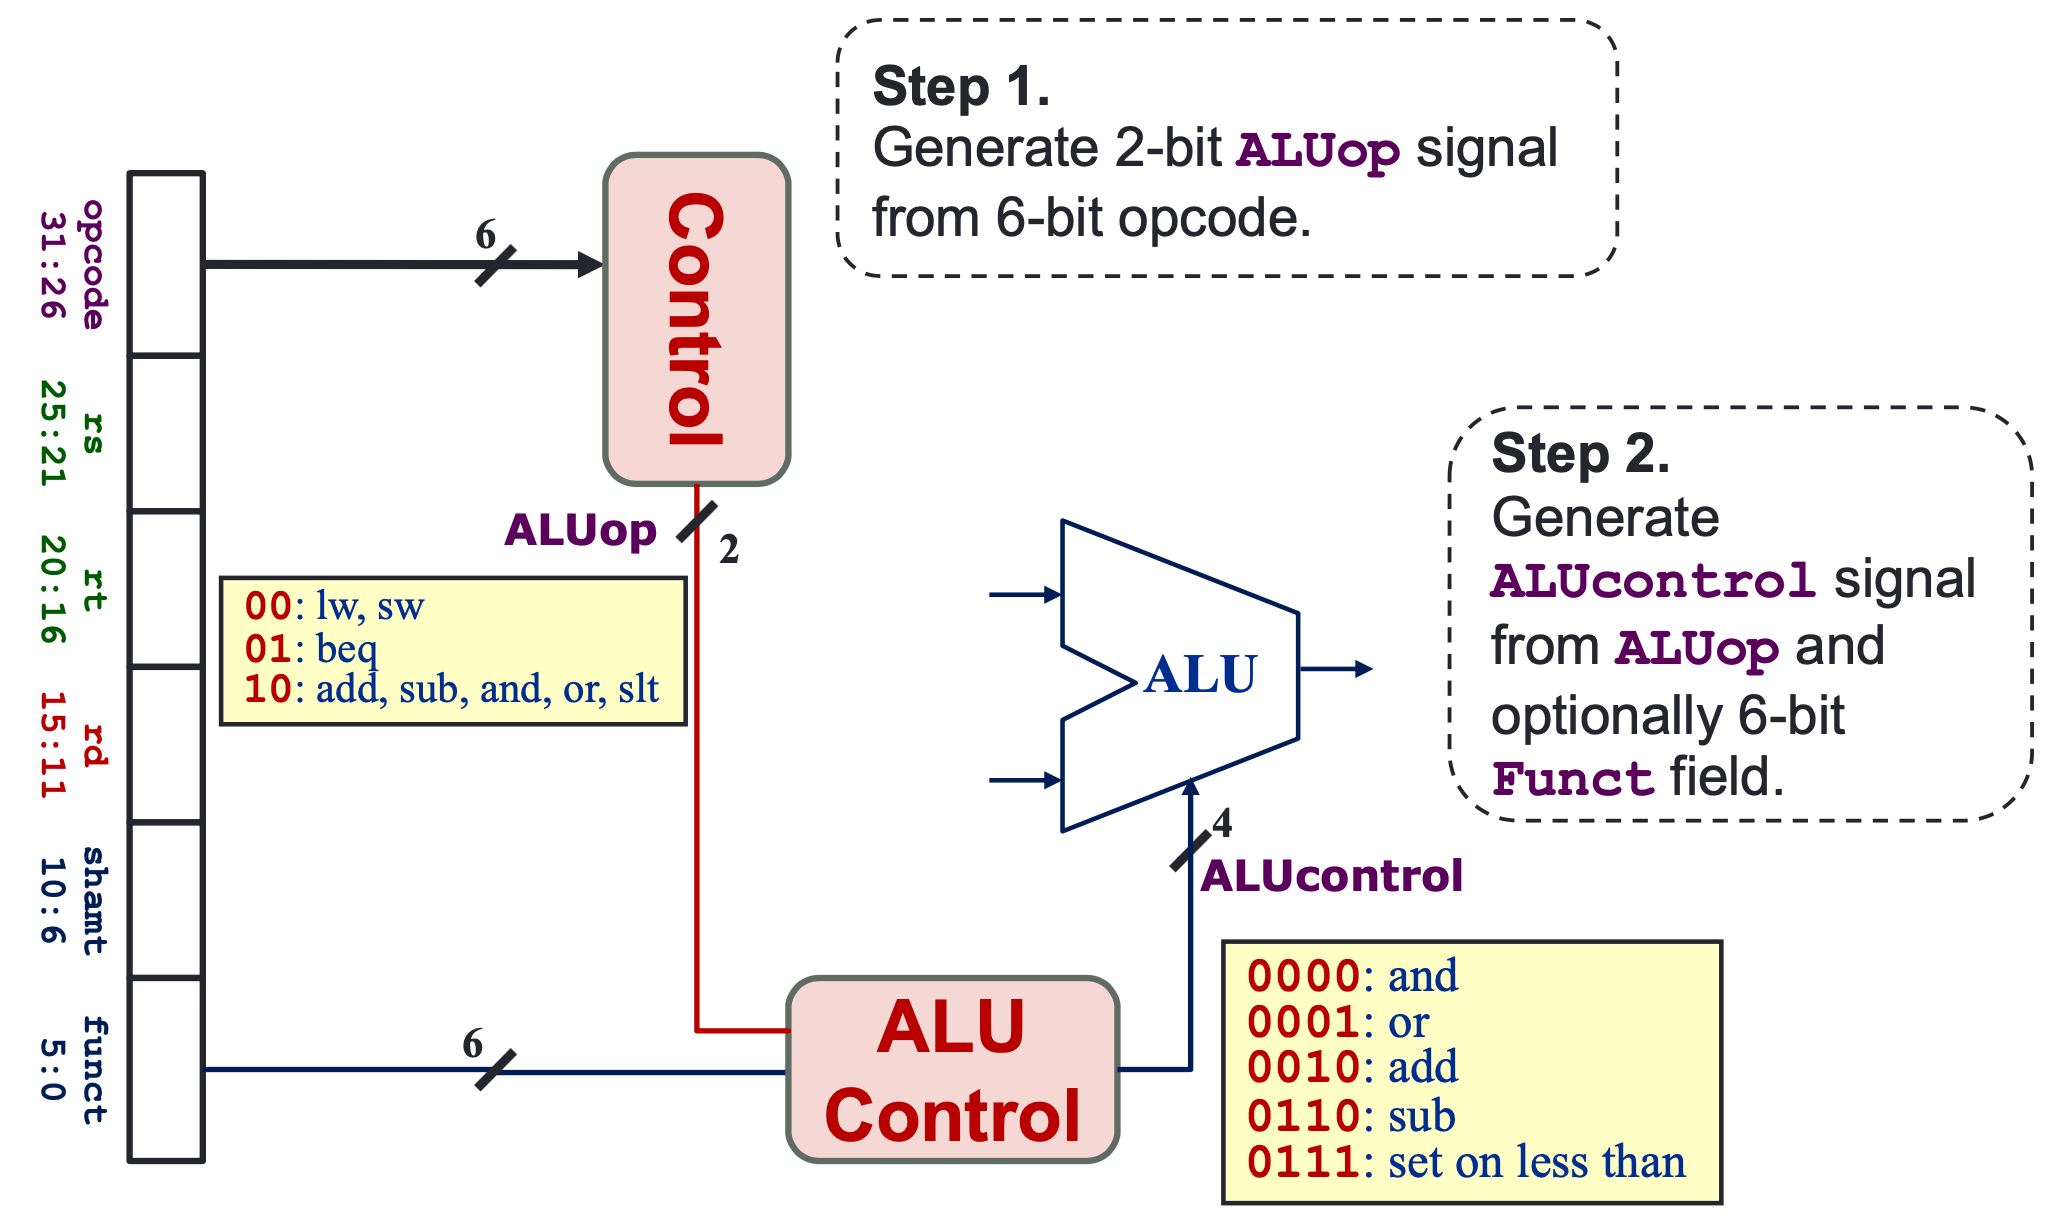
\includegraphics[scale=0.25]{./assets/ALUop}\\
		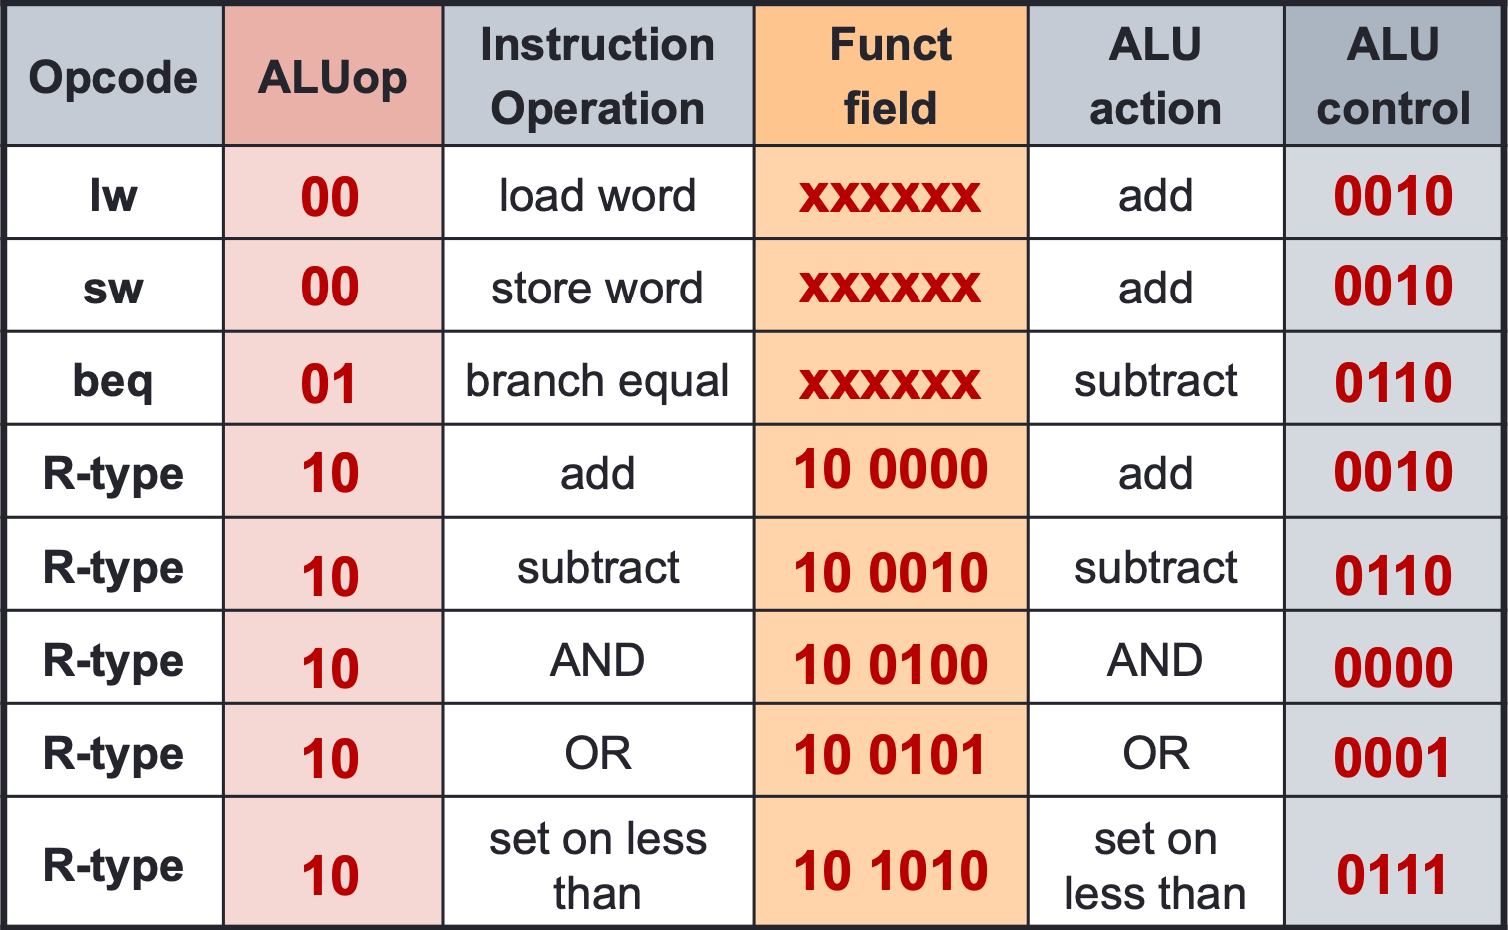
\includegraphics[scale=0.25]{./assets/ALUControlTable}\\
		- Table of Opcode, funct field and corresponding ALUop and ALUcontrol signals\\
		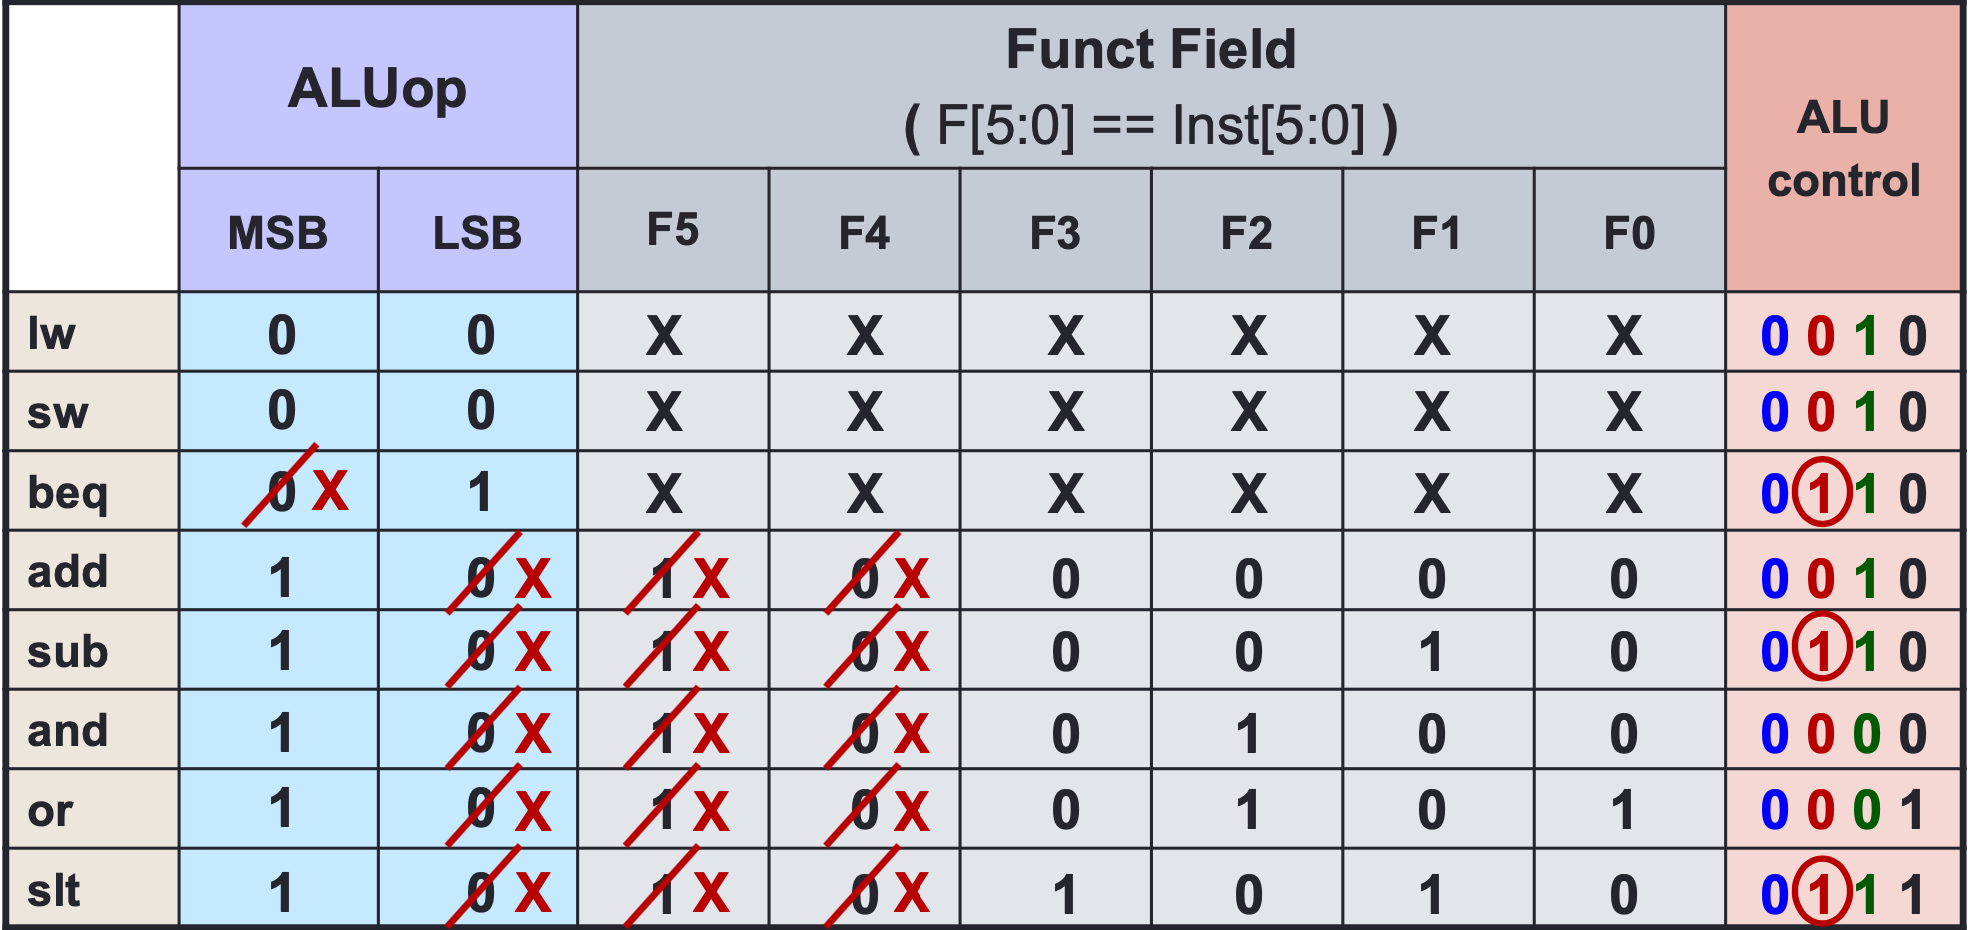
\includegraphics[scale=.25]{./assets/ALUControlTable2}\\
		- Table of how to generate each bit of ALUControl\\
		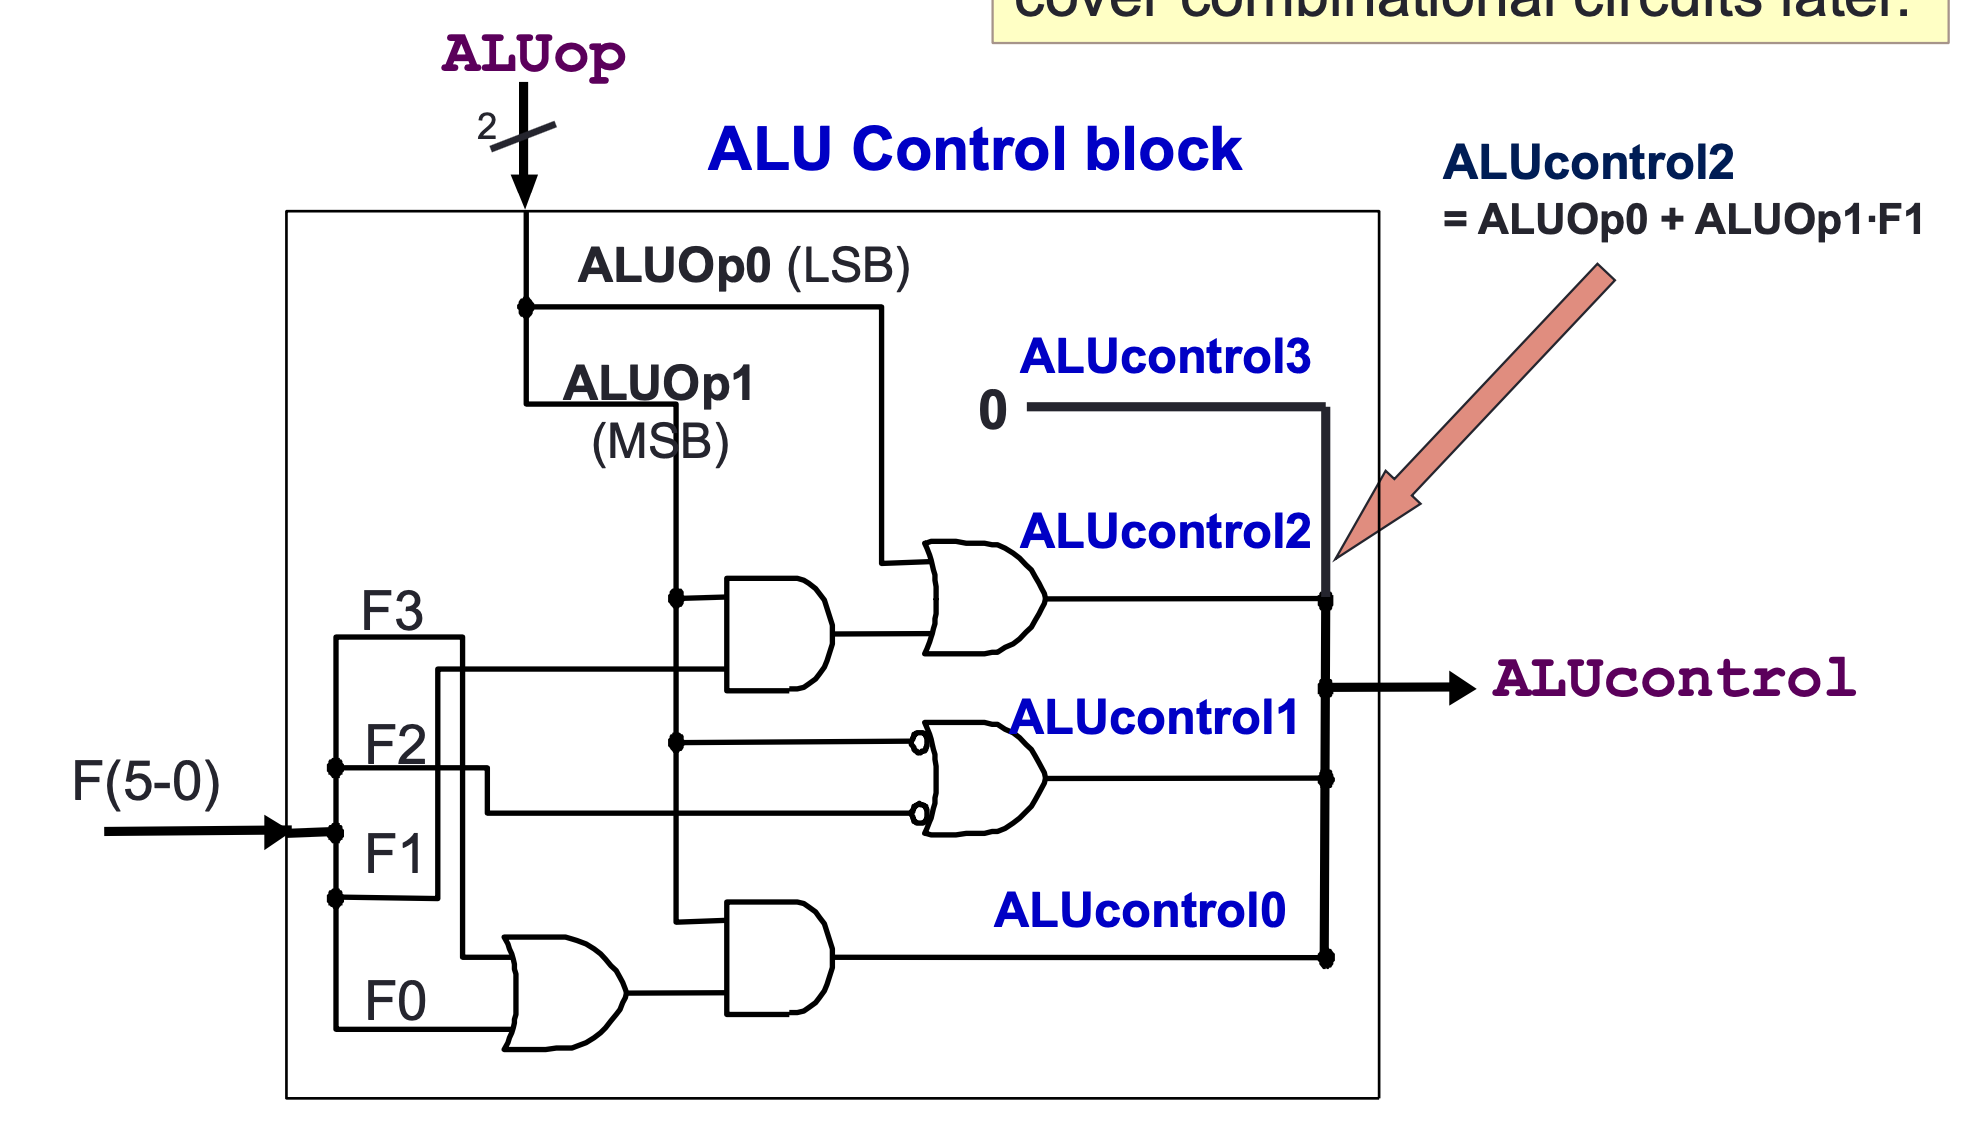
\includegraphics[scale=.25]{./assets/ALUControlBlockCircuit}\\
		- Circuit of ALUControl Block\\
		$ALUControl0 = (ALUop_1 \cdot F_3) + (ALUop_1 \cdot F_0) = ALUop_1 \cdot (F_0 + F_3)$\\
		$ALUControl1 = (ALUop_1 \cdot F_2)'$\\
		$ALUControl2 = ALUop_0 + ALUop_1 \cdot F_1$\\
		$ALUControl3 = 0$\\
		\textbf{Control Design}\\
		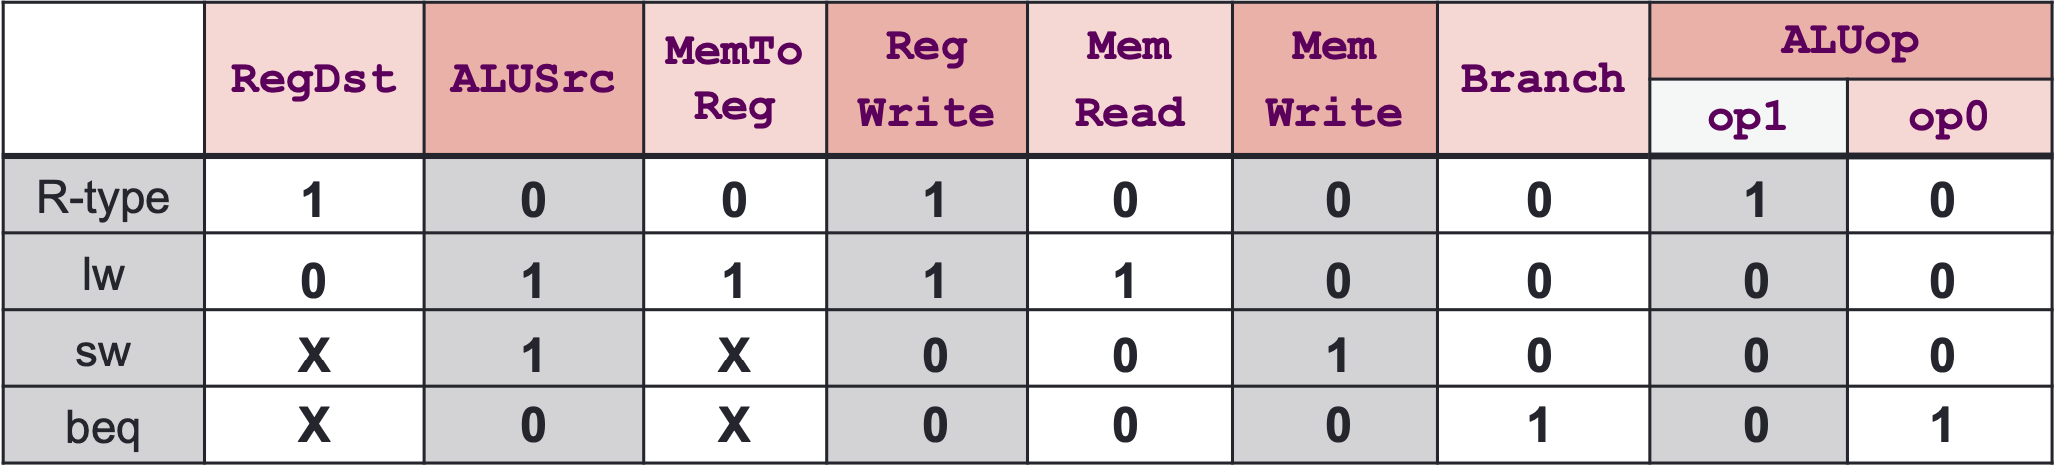
\includegraphics[scale=.25]{./assets/controlTable}\\
		- Table of control signals for various instructions (outputs)\\
		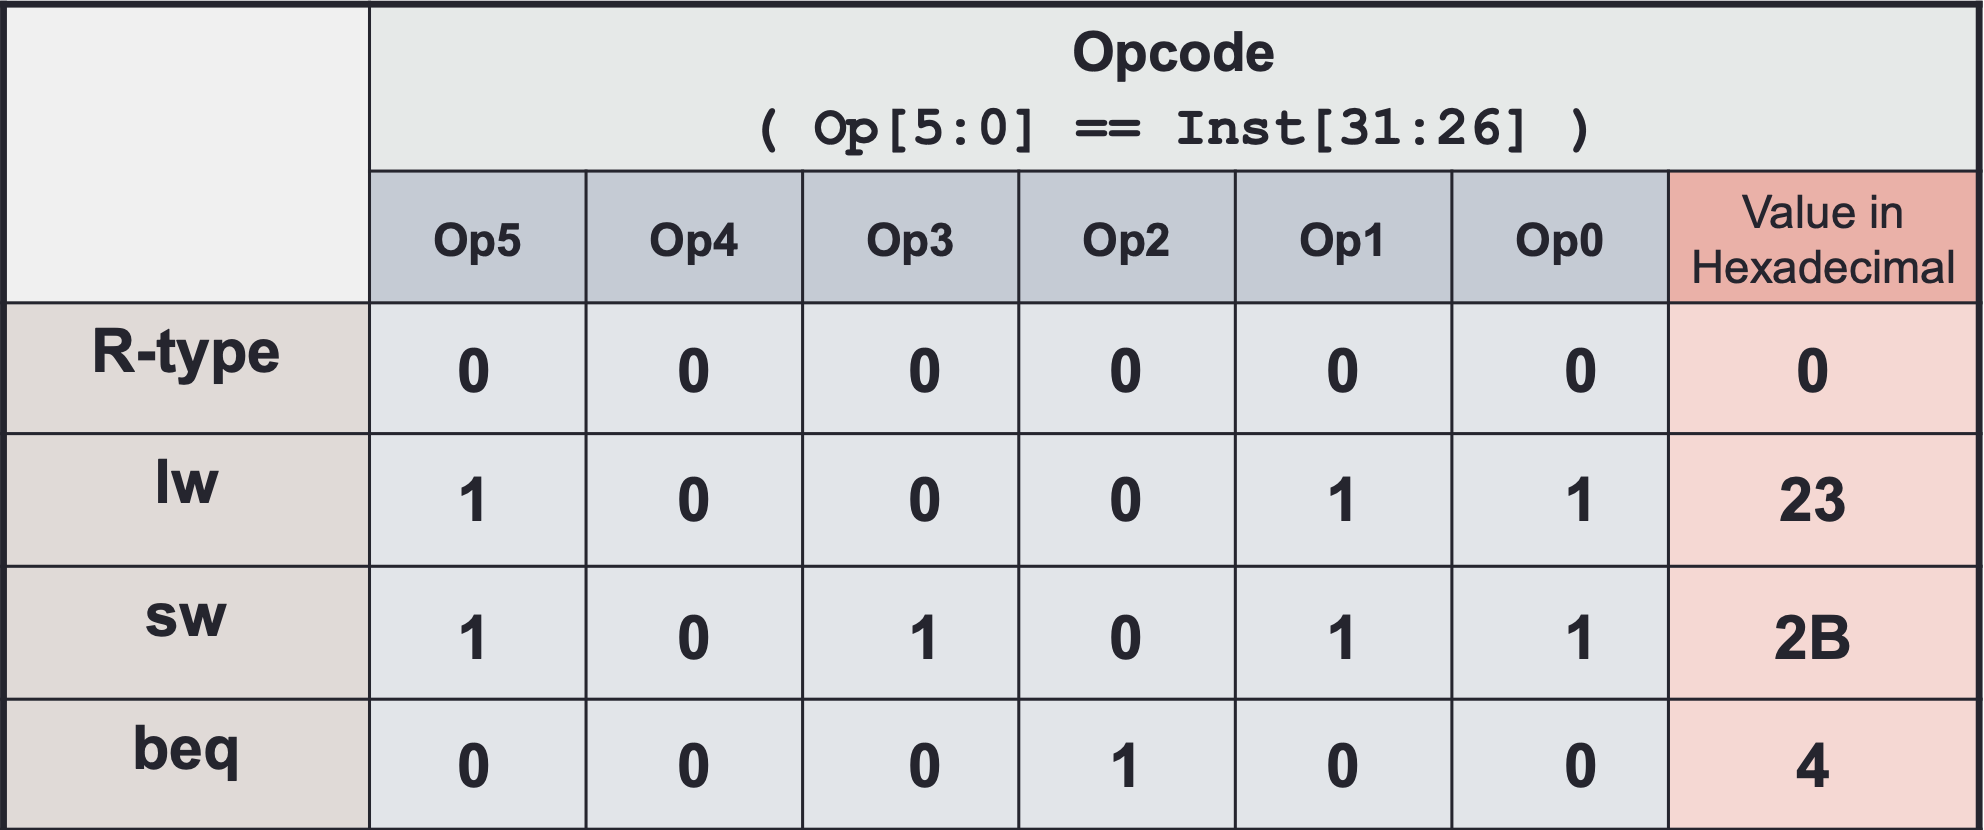
\includegraphics[scale=.25]{./assets/opcodeTable}\\
		- Table of opcode for the various types of instructions (inputs)\\
		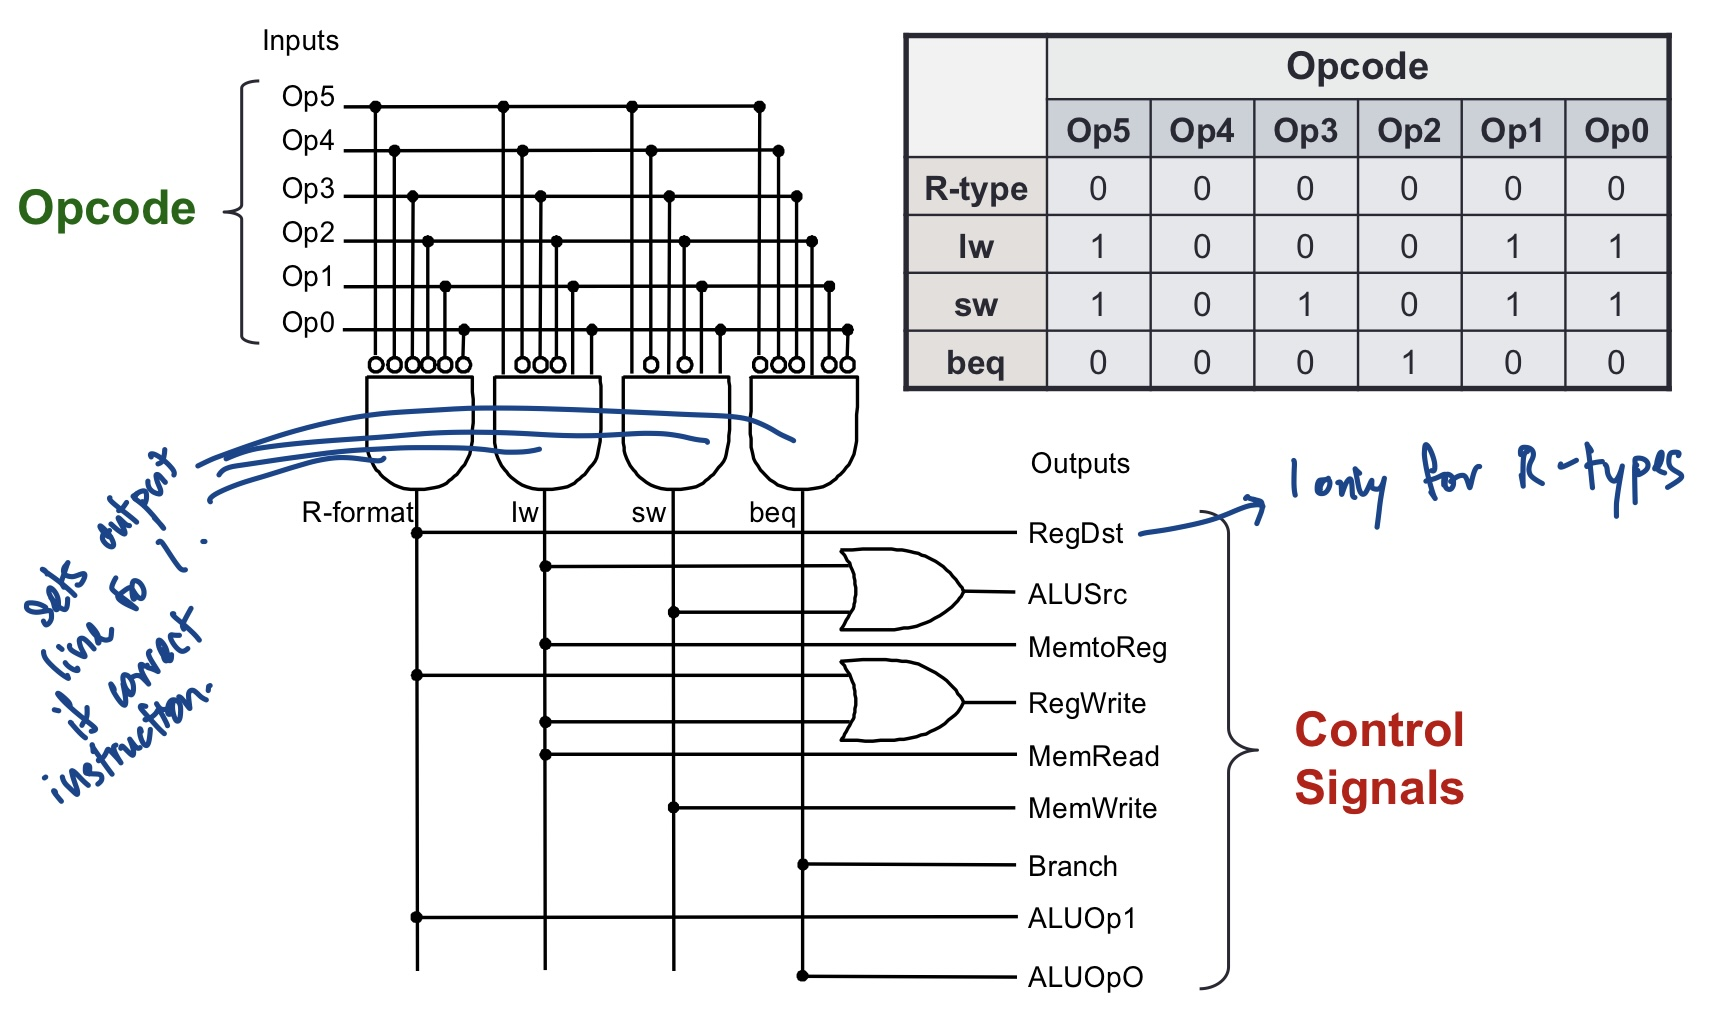
\includegraphics[scale=0.16]{./assets/controlCircuit}\\	
		
		\textbf{Instruction Execution}\\
		1. Read contents of register or memory\\
		2. Perform computation\\
		3, Write results\\
		Perform all within a clock period to prevent reading a storage element when it is being written\\
		
		\textbf{Single Cycle Implementation}\\
		- All instructions take one cycle\
		- Cycle must be at least as long as slowest instruction\\
		- All instructions take as much time as slowest instruction\\
		
		\textbf{Multicycle Implementation}\\
		- Break up instructions into execution steps (IF, ID, EX, MEM, WR)\\
		- Each execution step takes 1 clock cycle $\implies$ cycle time much shorter\\	
		- Cycle must be long enough to accomodate longest step\\
		- Each step takes as much time as longest step\\
		- Instructions take variable number of clock cycles to complete execution\\
		Not covered\\
		
		\textbf{Pipelining}\\
		- One step per clock cycle\\
		- Execute different steps of multiple instructions simultaneously\\
		
		{\normalsize\textbf{Boolean Algebra}}\\
		\textbf{Precedence of Operators}\\
		- Not (')\\
		- And (.)\\
		- Or (+)\\
		
		\textbf{Boolean Algebra Laws}\\
		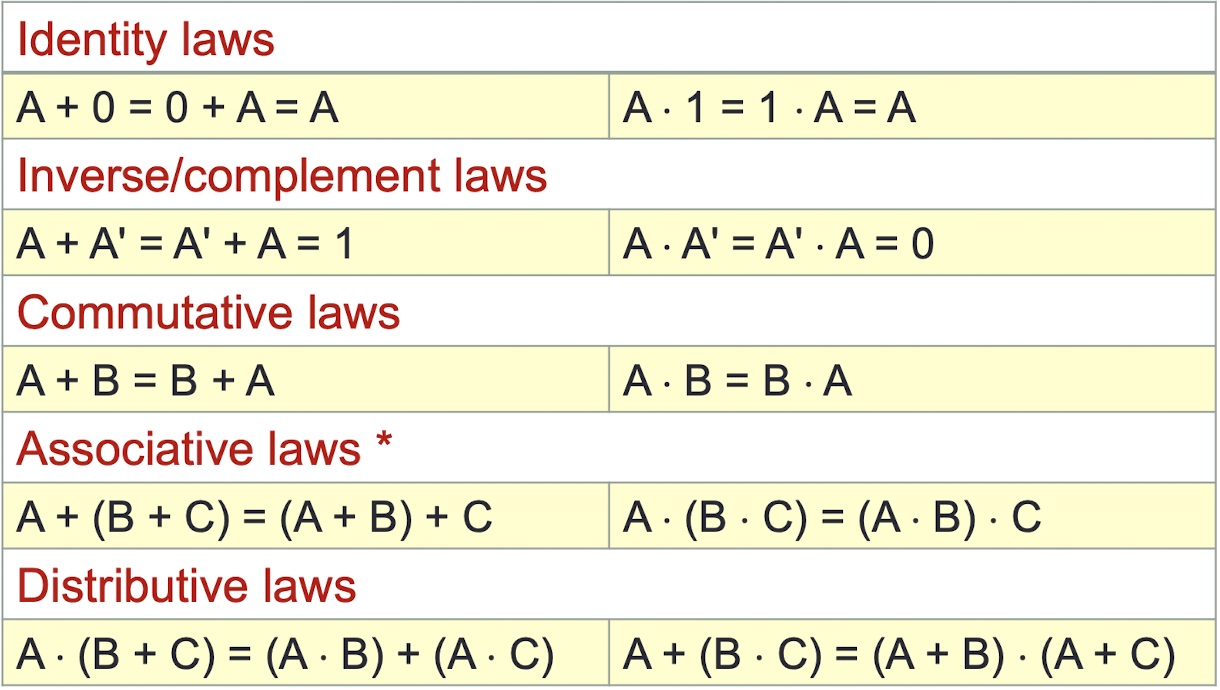
\includegraphics[scale=.35]{./assets/booleanAlgebraLaws}\\
		
		\textbf{Duality}\\
		If AND/OR operators and identity elements 0/1 in a Boolean Equation are interchanged, it remains valid\\
		
		\textbf{Theorems}\\
		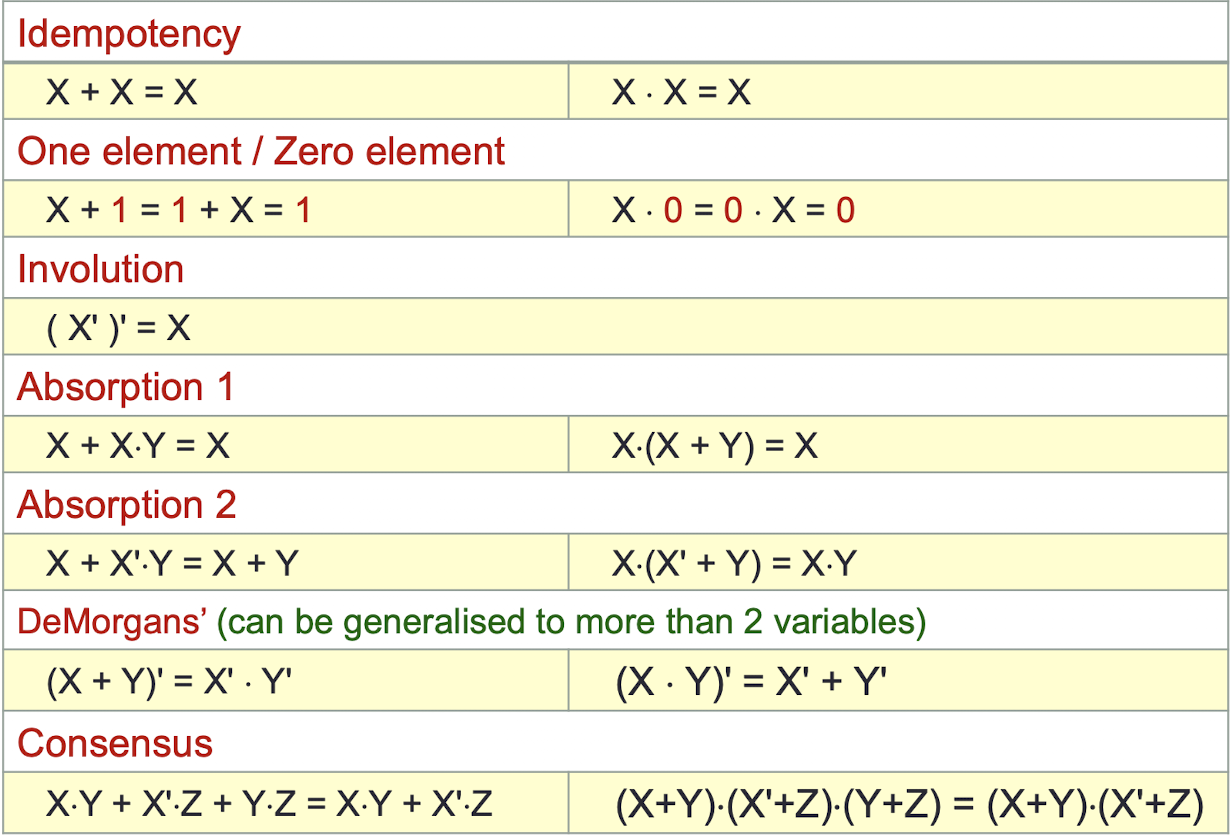
\includegraphics[scale=.35]{./assets/booleanAlgebraTheorems}\\
		
		\textbf{Standard Form}\\
		Every boolean expression can be expressed in SOP or POS.\\
		- Literals: Boolean variable or complemented form, eg. \texttt{x or x'}\\
		- Product Term: single literal or a product (AND) of several literals, eg \texttt{x or x.y.z'}\\
		- Sum Term: single literal or a sum (OR) or several literals, eg \texttt{x or x+y+z'}\\
		- Sum-of-Products (SOP): product term or sum (OR) of product terms, eg \texttt{x, x.y.z', x + y.z,}\\
		- Product-of-Sum (POS): sum term or product (AND) of sum terms, eg \texttt{x, x+y+z', x.(x+y)}\\
		
		\textbf{Minterm and Maxterm}\\
		- Minterm of \textit{n} variables is a \textbf{product term} that contains \textit{n} literals from all the variables\\
		eg. for two variables \texttt{x, y}, minterms are \texttt{x'.y', x'.y, x.y', x.y}\\
		- Maxterm of \textit{n} variables is a \textbf{sum term} that contains \textit{n} literals from all the variables.\\
		eg. for two variables \texttt{x, y}, maxterms are \texttt{x'+y', x'+y, x+y', x+y}\\
		
		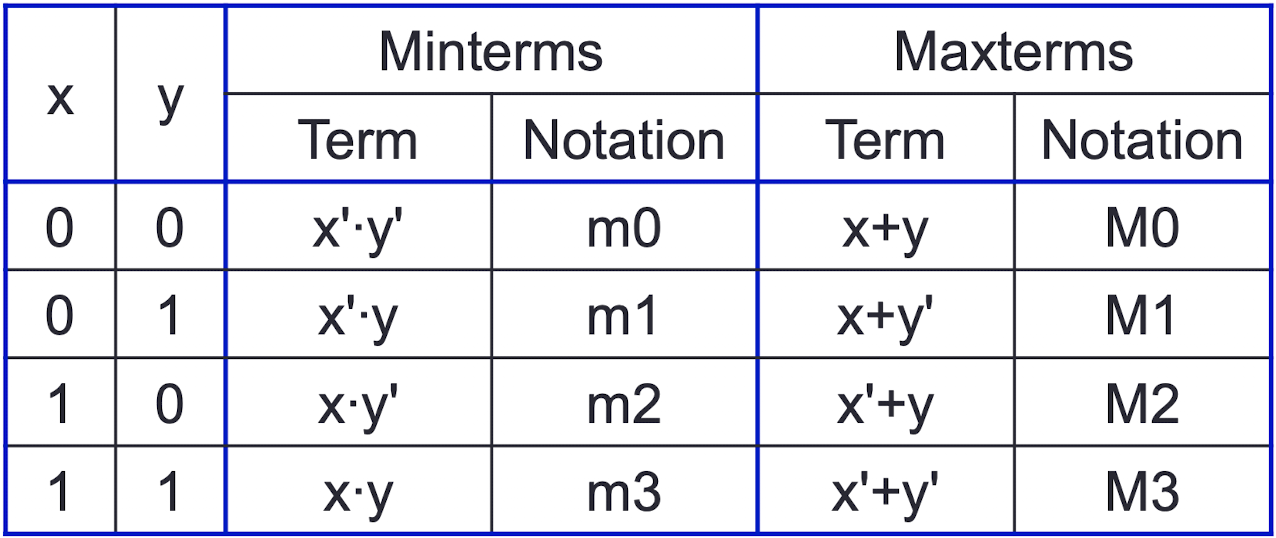
\includegraphics[scale=.35]{./assets/mintermAndMaxterm}\\
		
		\highlight{Note}: Each minterm is the compement of its corresponding maxterm, and vice-versa\\

		Given truth table\\
		- Obtain \textbf{sum of minterms} by gathering minterms (where output is 1)\\
		- Obtain \textbf{product of maxterms} by gathering maxterms (where output is 0)\\
		
		Conversion between standard forms\\
		\textbf{sum of minterm} $\rightarrow$ \textbf{product of max terms}\\
		-eg $F2 = \sum m(1,4,5,6,7) = \prod M(0,2,3)$\\
		
		{\normalsize\textbf{Logic Circuit}}\\
		SOP expression can be implemented using\\
		- 2-level AND-OR circuit\\
		- 2-level NAND circuit\\
		
		POS expression can be implemented using\\
		- 2-level OR-AND circuit\\
		- 2 level NOR circuit\\
		
		{\normalsize\textbf{Simplification}}\\
		- Algebraic: using theorems\\
		- K-map: no more than 6 variables\\
		- Quine-McClusky: non-examinable\\
		
		\textbf{Gray Code}\\
		- Unweighted\\
		- Only a \textbf{single bit change} from one code value to the next\\
		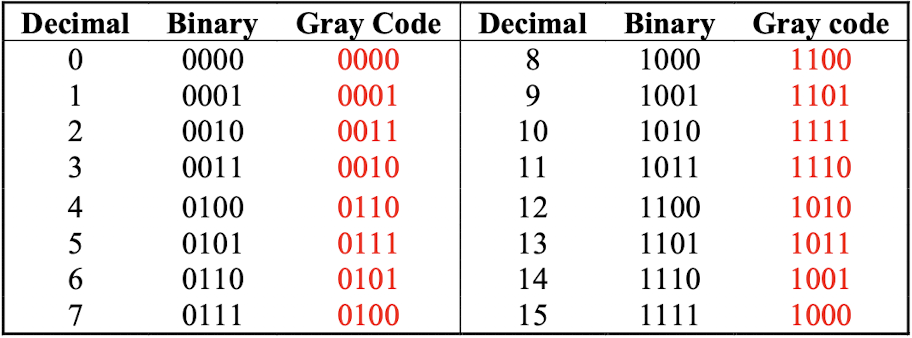
\includegraphics[scale=.4]{./assets/grayCode}
		
		\textbf{K-maps}\\
		- Limited to 5 or 6 variables\\
		- Each square represents a minterm\\
		- Two adjacent squares represent minterms that differs by exactly 1 literal\\
		- K-map of $n$ variables has $2^n$ squares, each cell has $n$ neighbors\\
		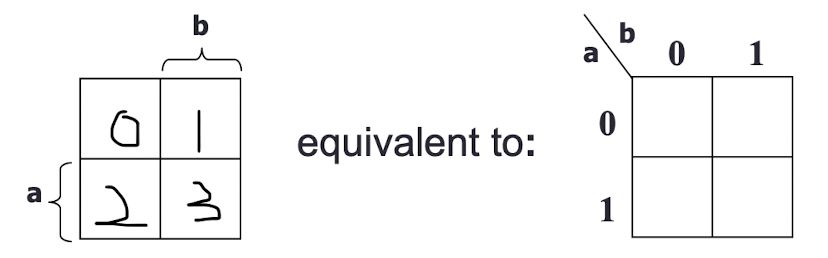
\includegraphics[scale=.3]{./assets/2VarKMap}\\
		\highlight{Note}: there is wrap-around in kmaps\\
		
		\textbf{How to use K-Map}\\
		- Group as many cells together as possible: larger group $\rightarrow$ less literals\\
		- As few groups to cover all 1s: fewer groups $\rightarrow$ fewer product terms\\
		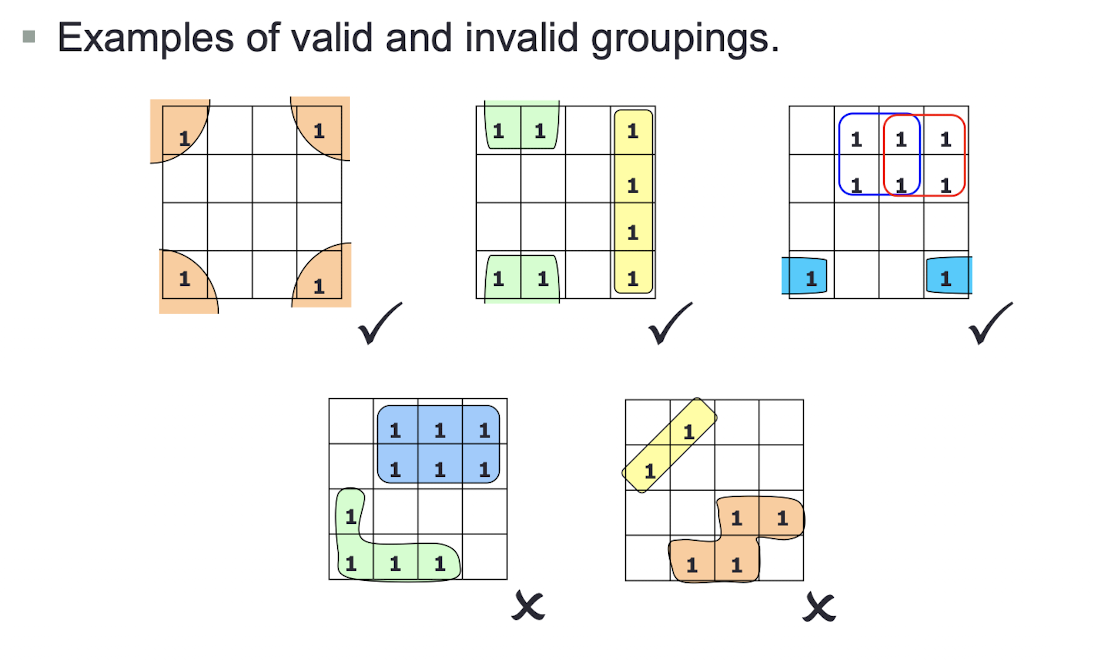
\includegraphics[scale=.35]{./assets/validInvalidGroupings}
		
		\textbf{PI and EPI}\\
		Prime Implicant: product term obtained by combining the \highlight{maximum possible number of minterms} from adjacent squares, biggest group.\\
		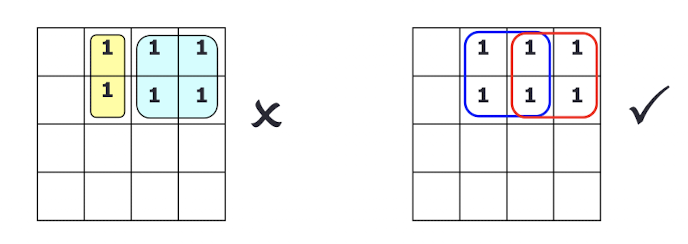
\includegraphics[scale=.4]{./assets/primeImplicant}

		Essential Prime Implicant: A prime implicant that includes \highlight{at least one minterm not covered} by any other PIs.\\
		Reduces number of redundant groups.\\
		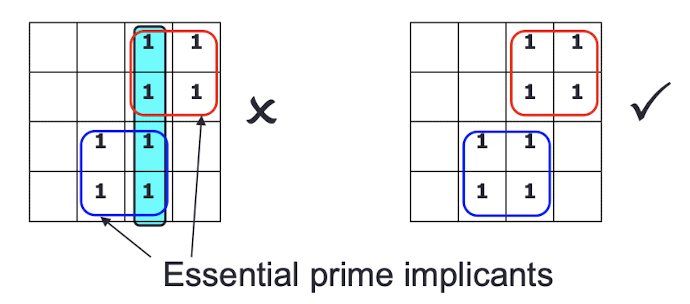
\includegraphics[scale=.4]{./assets/EPI}
		
		\textbf{Algorithm for SOP}\\
		1. Find PIs\\
		2. Find EPIs\\
		3. Choose all EPIs\\
		4. Choose PIs that cover minterms not covered by EPIs\\
		
		\textbf{Algorithm for POS}\\
		1. Same as SOP, but group maxterms (0s) instead
		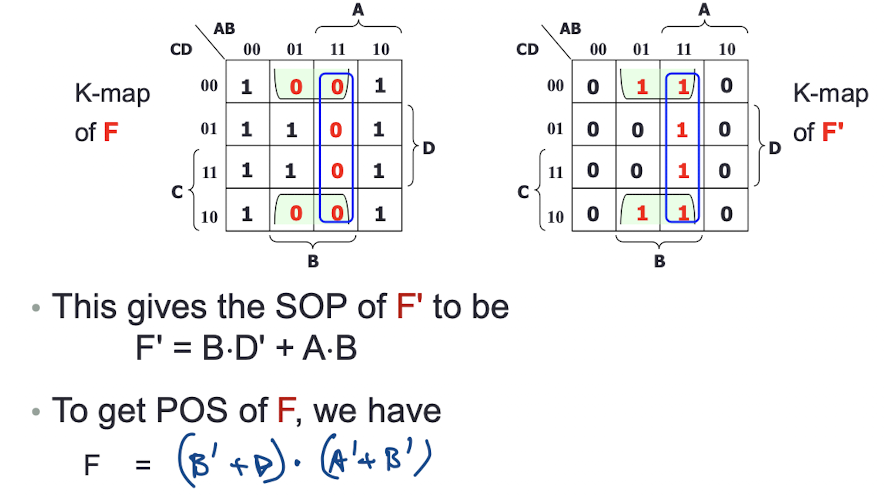
\includegraphics[scale=.45]{./assets/POSKmap}
		
		\textbf{Don't Care Conditions}\\
		- If output is not specified or invalid, it can be 0 or 1, and are denoted by X or d.\\
		- Can be chosen to be either 1 or 0 to make a simpler SOP or POS expression.\\

		{\normalsize\textbf{MSI Components}}\\
		Medium Scale Integration\\

		\textbf{Decoder}\\
		Chooses one (of $2^n$) output lines based on $n$ input lines. \\
		Each output corresponds to minterm of the $n$ functions\\
		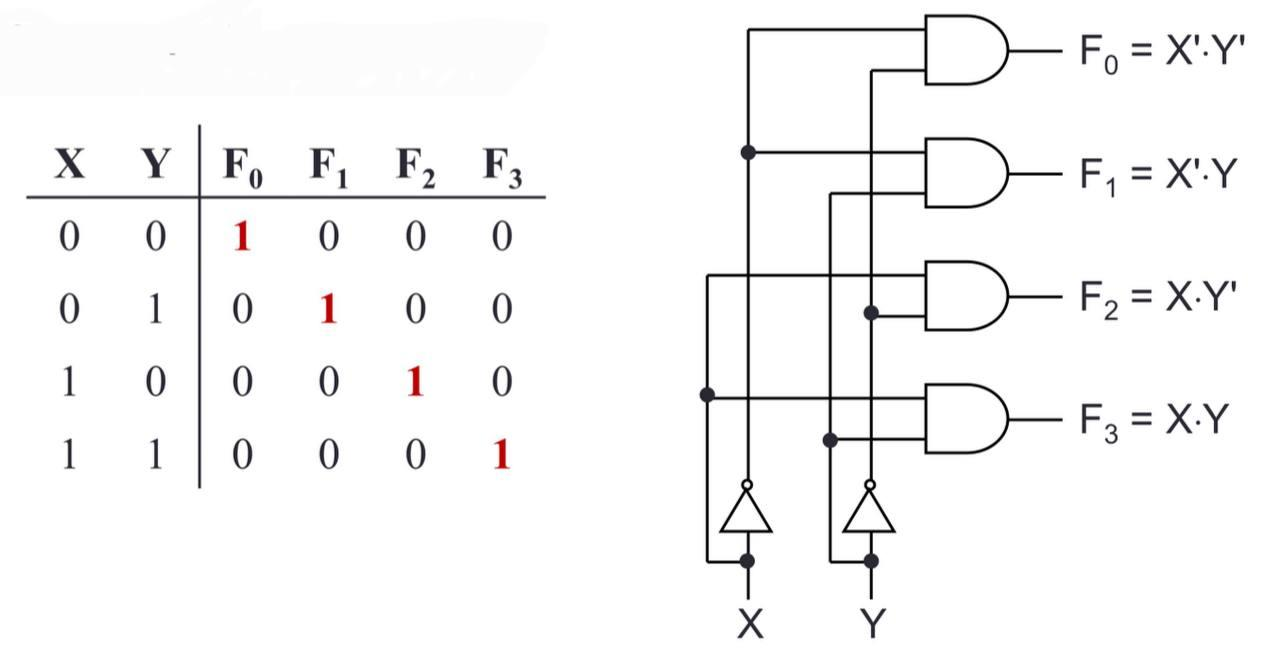
\includegraphics[scale=.18]{./assets/decoder}

		Decoder with enable\\
		- output 0 when disabled, E = 0 in one enabled decoder\\

		Active Low decoder\\
		- selected line = 0, other lines 1\\
		- implement function using NAND instead\\

		Larger decoders can be constructed from smaller decoders and inverter using one of the inputs as enable signal\\

		Implementing functions\\
		- use decoder to generate minterms or maxterms\\
		- inputs as selector lines to choose minterms or maxterms\\
		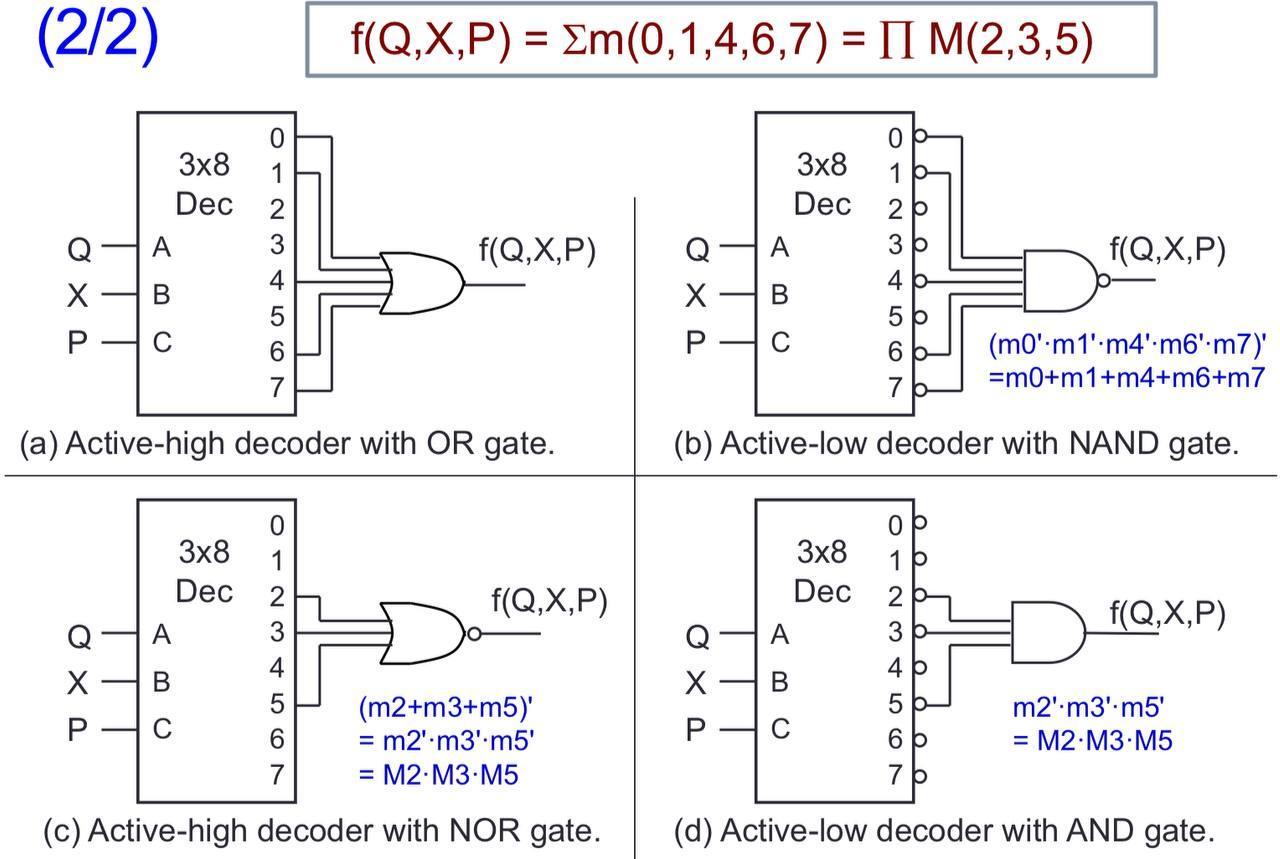
\includegraphics[scale=.23]{./assets/decoderFunctions}

		\textbf{Encoder}\\
		- only one input = 1, returns the corresponding number of the input.\\
		- Opposite of decoder\\

		Priority Encoder\\
		- Encoder output depends only on MSB, can have $ > 1$ input line = 1\\

		\textbf{Demultiplexer}\\
		- Directs data from input line to one of the output lines, depending on the selector lines\\
		- Circuit is same as decoder with enable, data input -> enable, selector lines -> decoder input\\

		\textbf{Multiplexer}\\
		Directs one of $2^n$ inputs to a single output line, using $n$ selector lines. Known as a \red{data selector}\\
		- output is the sum of (product of data lines and selection lines)\\
		- $Output = I_0 \cdot (S_1' \cdot S_0') + I_1 \cdot (S_1' \cdot S_0) + I_2 \cdot (S_1 \cdot S_0') + I_3 \cdot (S_1 \cdot S_0)$\\
		- $Output = I_0 \cdot m_0 + I_1 \cdot m_1 + I_2 \cdot m_2 + I_3 \cdot m_3$\\

		Implementing Functions with Multiplexers\\
		1. Express function in sum-on-minterm form\\
		2. Connect $n$ variables to $n$ selector lines\\
		3. Connect $1$ to data line if it is a minterm of function or $0$ otherwise\\
		\highlight{Note}: Can use smaller multiplexers\\
		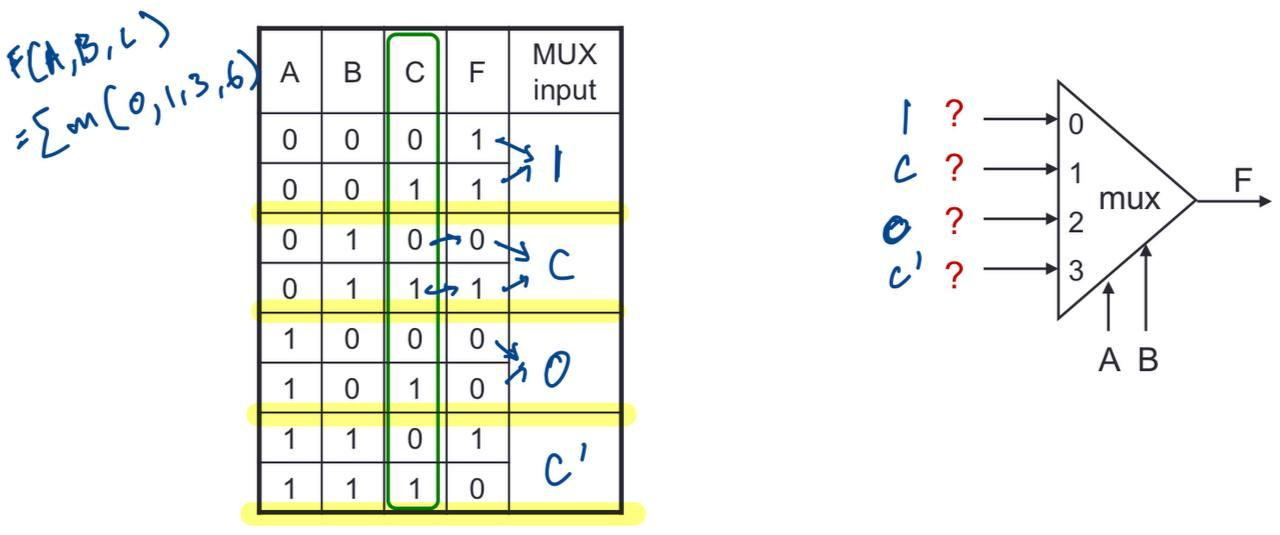
\includegraphics[scale=.2]{./assets/smallerMux}

		{\normalsize\textbf{Sequential Logic}}\\
		Two types of sequential circuits\\
		- Synchronous: outputs change only at specific time\\
		- Asynchronous: outputs change at any time
		Multivibrator: a class of sequential circuits\\
		- Bistable (2 stable states)\\
		- Monostable or one-shot (1 stable state)\\
		- Astable (no stable state)\\
		Bistable Logic devices\\
		- \textbf{Latches and Flip-Flops}\\
		- Latches: pulse triggered\\
		- Flip-flops: edge triggered\\
		\textbf{S-R Latch}\\
		Two inputs: $S$ and $R$\\
		Two complementary outputs: $Q$ and $Q'$\\
			- When $Q$ = 1, in \highlight{SET} state\\
			- When $Q$ = 0, in \highlight{RESET} state\\
		For Active High S-R Latch\\
			- R = 1. S = 0: RESET\\
			- R = 0, S = 1: SET\\
			- R = 0, S = 0: No change\\
			- R = 1, S = 1: invalid\\
		For Active Low S-R Latch\\
			- flip\\
		Gated Latches\\
			- Enable input $EN$ changes only if $EN$ is HIGH\\
		\textbf{D Latch}\\
		- Same as SR Latch without invalid condition and only 1 input\\
		- Single input D, D sent to S input, negated D sent to R input\\
		- $Q^+ = D$\\

		\textbf{Flip Flops}\\
		Change state at rising or falling edge of clock signal\\
		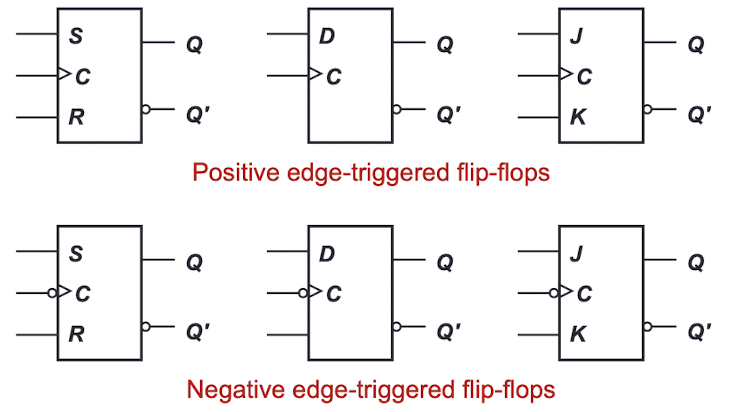
\includegraphics[scale=.4]{./assets/flipflops}
		
		\textbf{J-K Flip-flop}\\
		$Q$ and $Q'$ are fed back to the pulse-steering NAND gates.\\
		- No invalid state: when $J$ and $K$ are 1 $\rightarrow$ \highlight{Toggle}\\
		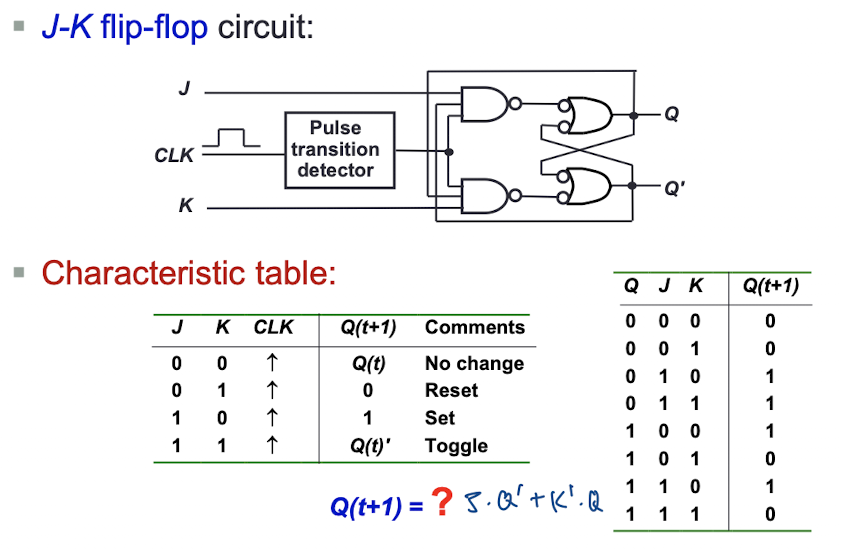
\includegraphics[scale=.5]{./assets/JKFlipFlop}
		
		\textbf{T Flip-flop}\\
		Single input version of the J-K flip-flop, tie both input together\\
		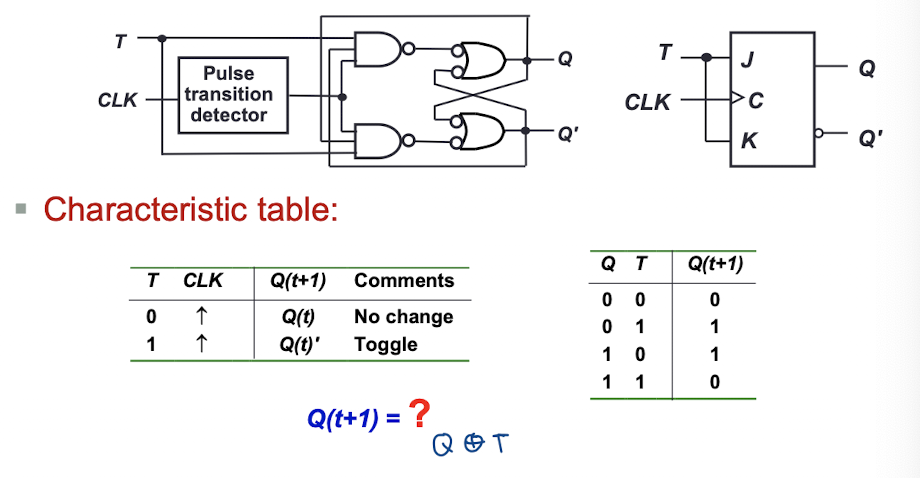
\includegraphics[scale=.5]{./assets/TFlipFlop}
		
		\textbf{Asynchronous Inputs}\\
		Affect state of flip-flop independent of clock\\
		- $PRE = 1$, Q is \highlight{immediately} set to 1\\
		- $CLR = 1$, Q is \highlight{immediately} set to 0\\
		- $PRE = 0, CLR = 0$, normal flip-flop operation\\
		
		\textbf{Characteristic Table (for analysis)}\\
		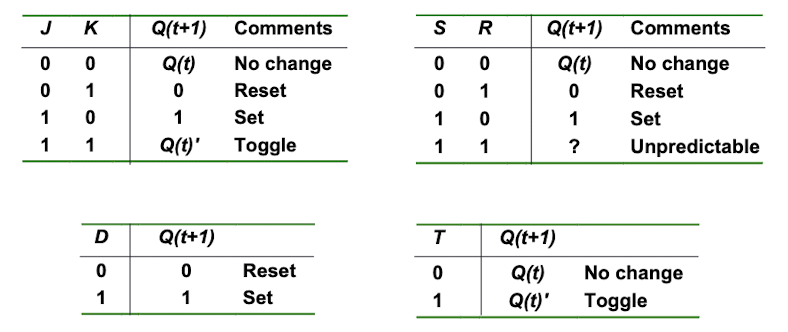
\includegraphics[scale=.6]{./assets/CharacteristicTable}
		
		\textbf{Analysis of Sequential Circuit}\\
		1. Derive state equations / input equations from ff inputs, and output functions (if 
		any)\\
		2. Derive state table and hence diagram, using state equations and characteristic table\\
		
		\textbf{Excitation Table (for Design)}\\
		Excitation Tables: given the required transition from present state to next state, determine the flip-flop inputs\\
		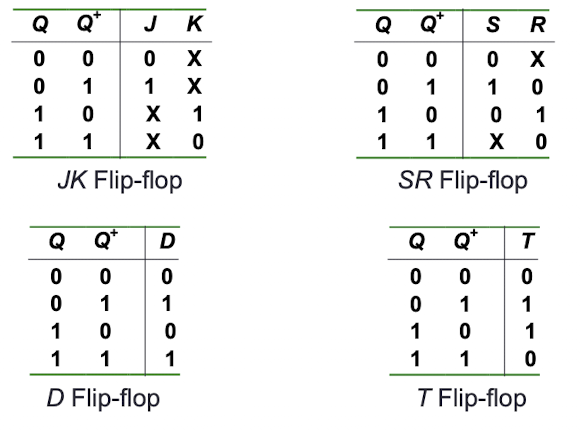
\includegraphics[scale=.6]{./assets/excitationTables}
		
		\textbf{Design Procedure}\\
		1. Start with specs - state diagram or state table.\\
		2. Derive state table\\
		3. Perform state reduction if necessary\\
		4. Perform state assignment\\
		5. Determine number of flip-flops and label them.\\
		6. Choose type of flip-flop\\
		7. Derive Circuit excitation and output tables from the state table\\
		8. Derive circuit output functions and flip-flop input functions (simplify w kmap if necessary)\\
		9. draw logic diagram\\
		
		{\normalsize\textbf{Pipelining}}\\
		Pipelining doesn't help latency of single task, but helps throughput of entire workload\\
		Multiple tasks operating simultaneously using different resources\\
		Delays\\
		- limited by slowest pipeline stage\\
		- stall for dependencies\\
		
		\textbf{MIPS Pipeline}\\
		Five pipelining stages\\
		- \highlight{IF}: Instruction Fetch\\
		- \highlight{ID}: Instruction Decode and Register Read\\
		- \highlight{EX}: Execute operation or calc address (ALU)\\
		- \highlight{MEM}: Read/Write from/to memory\\
		- \highlight{WB}: Write back the result into a register\\
		
		Each execution stage takes 1 clock cycle\\
		General flow of data is from one stage to the next\\
		
		Exception: Update of PC and write back to reg file\\
		
		\textbf{Pipeline Datapath}\\
		Data used by \highlight{same instruction} in later pipeline stages need to be stored somewhere (due to multicycle(?))\\
		- Additional registers in datapath called \highlight{pipeline registers}\\
		- \texttt{IF / ID}: Register between \texttt{IF} and \texttt{ID}\\
		- \texttt{ID / EX}: Register between \texttt{ID} and \texttt{EX}\\
		- \texttt{EX / MEM}: Register between \texttt{EX} and \texttt{MEM}\\
		- \texttt{MEM / WB}: Register between \texttt{MEM} and \texttt{WB}\\
		No need for register at end of \texttt{WB} stage as it is the end of the command.\\
		\highlight{Note:} Need to send the "Write Register" number along through the pipeline registers so that it can be used in \texttt{WB} stage\\
		
		\textbf{Pipeline Control}\\
		Difference from single-cycle datapath: Each control signal belongs to a particular pipeline stage\\
		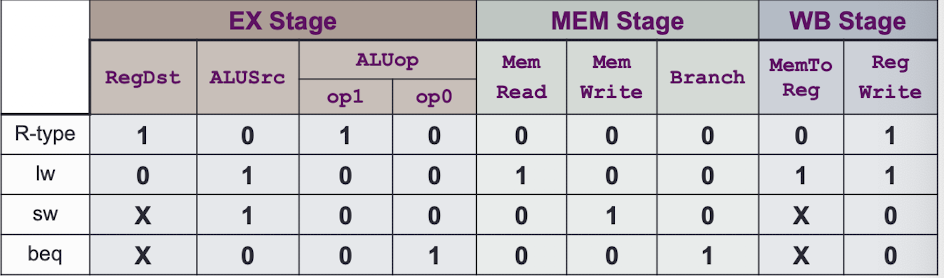
\includegraphics[scale=.5]{./assets/groupedControls}
		
		\highlight{Number of cycles needed in Idea pipeline}, with $I$ instructions:\\
		$I + N - 1$ in an N cycle pipeline (need $N-1$ cycles to fill pipeline)\\ 

		Pipeline processor can gain N times speedup, where N is the number of pipeline stages (ideal pipeline)\\
		
		{\normalsize\textbf{Pipeline Hazards}}\\
		Problems that prevent next intruction from immediately following previous instruction\\
		1. Structural hazards: Simultaneous use of hardware\\
		2. Data hazards: Data dependencies between instructions\\
		3. Control hazards: Change in program flow\\
		2 and 3 are Instruction Dependencies (instructions have relationships that prevent pipeline execution)\\
		
		\textbf{Structural Hazards}\\
		1. \texttt{IF} and \texttt{MEM} both access memory, clash between Inst 1 and 3\\
		\highlight{Solution}: Split memory into Data Memory and Instruction Memory.\\
		
		2. \texttt{ID} and \texttt{WB} both use reg file\\
		\highlight{Solution}: Registers are fast; Split cycle into two, write in first half, read in second half\\
		
		\textbf{Data dependency: RAW}\\
		Read-After-Write: Occurs when a later instruction \highlight{reads} from the destination register \highlight{writter} by an earlier instruction\\
		\highlight{Solution}: \highlight{Forward} the result to any later instruction before it is reflected in the register file. Replace data read from reg file of later inst.\\
		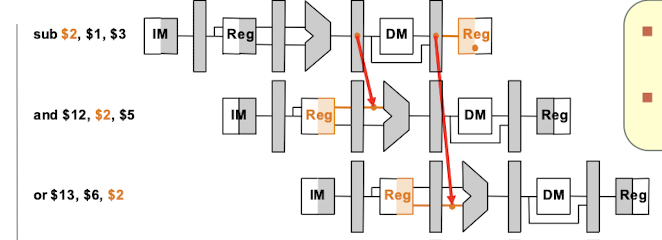
\includegraphics[scale=.7]{./assets/dataForwarding}
		
		\highlight{Exception}: \texttt{lw} cannot be solved with forwarding. Data is produced in \texttt{MEM}. Must stall 1 cycle\\
		In general, without data forwarding stall \highlight{2} cycles (3 if \texttt{lw} is preceding).\\
		
		\textbf{Control Dependency}\\
		Definition: An instruction \texttt{j} is control dependent on \texttt{i} if \texttt{i} controls whether or not \texttt{j} executes. (branch inst)\\
		
		\highlight{Problem}: Branch Decision is made at \texttt{MEM} stage.\\
		\highlight{Solution}: \\
		1. Stall the pipeline for 3 cycles.\\
		2. Early Branching: move the branch decision to an earlier stage\\
		3. Branch Prediction: Guess outcome of branch\\
		4. Delayed Branching: Do something useful while waiting for outcome\\
		
		\textbf{Early Branching}\\
		Make decision in \texttt{ID} stage instead of \texttt{MEM}\\
		- Move branch target address calculation\\
		- Move register comparison $\rightarrow$ cannot use \texttt{ALU} for register comparison any more\\
		- Still need to stall 1 cycle\\
		\highlight{NOTE} if register involved in comparison is produced by preceding instruction (RAW), need to stall \highlight{extra 1} cycle (total 2 cycles)\\
		If preceding instruction is \highlight{lw}, need to stall \highlight{extra 2} cycles $\rightarrow$ back to 3 cycles of delay\\
		
		\textbf{Branch Prediction}\\
		Simplest prediction scheme: branch not taken\\
		\highlight{Not taken}: Guessed correctly $\rightarrow$ No pipeline stall\\
		\highlight{Taken}: Guessed wrongly $\rightarrow$ Wrong instructions in the pipeline $\rightarrow$ \textbf{Flush} successor instruction from the pipeline\\
		
		\textbf{Delayed Branching}\\
		Move \textbf{non-control dependent instructions} into the X slots following a branch (1 if early branching)\\
		- These instructions are executed \textbf{regardless} of branch outcome\\
		- Must have the same behaviour as original code
		\highlight{NOTE}: Unless branch prediction is used in which case wrong instruction \textbf{will be flushed!}\\
		
		Best Case Scenario:\\
		There is an instruction \textbf{preceding the branch} which \textbf{can be moved} into the delayed slot.\\
		- Program correctness must be preserved
		
		Worst Case Scenario
		No instruction can be found
		- no-op instruction instead (\texttt{nop})\\

		{\normalsize\textbf{Cache}}\\
		small but fast SRAM near CPU, makes slow main memory appear faster\\

		\textbf{Memory Hierarchy}\\
		Registers are in the processor, if operands are in memory, need to load them into processor, operate, store back.\\
		- Fast RAM -> expensive\\
		- Cheap RAM -> slow\\
		Therefore have small but fast memory near CPU, large but slow memory farther from CPU\\
		Keep frequently and recently used data in \highlight{smaller but faster} memory\\

		\textbf{Principle of Locality}\\
		Program accesses only a small portion of the memory address space within a small time interval\\
		Types of Locality\\
		1. Temporal Locality - If an item is referenced, it will tend to be referenced soon again\\
		2. Spatial Locality - If an item is referenced, nearby items will tend to be referenced soon\\
		Different locality for instruction and data\\

		\textbf{Terminology}\\
		- \green{Hit}: Data is in the cache\\
		- \green{Hit rate}: Fraction of memory accesses that hit\\
		- \green{Hit time}: Time to access cache\\
		- \red{Miss}: Data is not in cache\\
		- \red{Miss Rate}: 1 - \green{Hit Rate}\\
		- \red{Miss Penalty}: Time to replace cache block + \green{Hit Time}\\
		Hit time < Miss penalty\\
		\highlight{Average Access Time} = Hit rate x Hit time + (1 - Hit rate) x Miss penalty\\

		\textbf{Memory to Cache Mapping}\\
		\highlight{Cache Block}: Unit of transfer between memory and cache\\
		- Typically 1 or more words (spatial locality)\\

		Observations:\\
		1. $2^{N}$-byte blocks are aligned at $2^{N}$-byte boundaries\\
		2. Addresses of words within a $2^{N}$-byte block have identical $(32-N)$ MSB.\\
		3. Bits $[31:N] \rightarrow$ \highlight{block number}\\
		4. Bits $[N-1:0] \rightarrow$ \highlight{byte offset} within a block\\

		\textbf{Direct Mapped Cache}\\
		- Each Block has exactly one location to be mapped to in cache (known as the \highlight{cache index})\\
		- Multiple blocks may be mapped to the same location in cache\\
		- But each is uniquely identified by its tag\\
		\highlight{Tag} = block number / no. of cache blocks.\\

		\includegraphics[scale=.3]{./assets/DirectCacheBits}\\
		\highlight{Note}: For MIPS, the 2 LSB of the offset is byte number, next 2 bit are word number within the block.\\
		Word number within block tells you which words to bring into cache\\

		\textbf{Cache Structure}\\
		- Data block\\
		- Tag\\
		- Valid bit\\

		\textbf{Reading Data}\\
		Cache hit when Tag[index] = Tag[Memory Address] \highlight{and}
		Valid bit = 1\\
		\highlight{Note}: initially all valid bits = 0\\
		\includegraphics[scale=.22]{./assets/readCacheData}

		\textbf{Writing Data}\\
		Changing only memory or cache $\rightarrow$ cache and memory out of sync\\
		Two policies:\\
		1. Write-through cache: Write data to both cache and memory\\
		2. Write-back cache: Only write to cache, write to main memory when cache block is evicted\\

		\textbf{Write Through Cache}\\
		\red{Problems}: Writes slowly at the speed of main memory\\
		\green{Solution}: Put a write buffer between cache and memory; CPU write to cache and buffer, mem controller write to memory\\
		\textbf{Write Back Cache}\\
		\red{Problem}: Wasteful to write back every block that is evicted\\
		\green{Solution}: Add a 'Dirty Bit' to each block and only write to memory if dirty bit = 1\\

		\textbf{Types of Misses}\\
		1. \blue{Compulsory / Cold Misses}: On the first access to a block; the block must be brought into the cache\\
		2. \blue{Conflict / Collision Misses}: Occurs in SA cache and Direct Mapped cache; when several blocks are mapped to the same block/set\\
		3. \blue{Capacity Misses}: Occurs when blocks are discarded from cache as cache cannot contain all blocks needed\\
		\textbf{Handling Cache Misses}\\
		- \blue{Read Miss}: load block into cache, read from cache\\
		- \blue{Write Miss}: Write Allocate - Load block into cache, change word, write to main memory depending on write policy\\
		- \blue{Write Miss}: Write Around - Write \highlight{straight to main mem} without loading block into cache\\
		\includegraphics[scale=.22]{./assets/writeDataCache}

		\textbf{Block Size}\\
		Reduces cache miss rate (due to spatial locality) up to a point, then increases (due to lower number of blocks in cache)\\

		\textbf{Set Associative Cache}\\
		Solution to the problem that there are too many conflicts\\
		\blue{N-way Set Associative Cache} - Memory block can be placed in N locations in cache\\

		In 2-way SA cache\\
		- Cache is split into sets, each set contains 2 blocks.\\
		- Memory block is mapped to a unique set, and can be placed in either block\\
		$\rightarrow$ need to search \highlight{both blocks} when searching cache\\
		\includegraphics[scale=.3]{./assets/SACache}
		\highlight{Note}: Formula is similar to DM cache, but \highlight{Set Index} rather than \highlight{Index}\\

		\textbf{Advantage of Associativity}\\
		Rule of Thumb - A direct mapped cache of size N has about the same miss rate as a 2-way SA cache of size N/2\\

		\textbf{Fully Associative Cache}\\
		Memory block can be placed in any location in cache\\
		\green{Pros}: Can be placed in any location in cache\\
		\red{Cons}: Need to search all of the locations in cache for a block\\
		\includegraphics[scale=.28]{./assets/FACache}\\
		\highlight{Note}: No conflict misses but have capacity misses\\

		\textbf{Cache Performance}\\
		1. Compulsory/Cold misses remain same irrespective of cache size and associativity\\
		2. Conflict Misses decrease with increasing associativity\\
		3. Conflict Misses = 0 for FA cache\\
		4. Capacity Misses decrease with cache size\\

		\textbf{Block Replacement Policy} (for SA and FA cache)\\
		Least Recently Used (LRU) policy:\\
		- \blue{How}: for each cache hit, record the cache block that was accessed. When replacing, choose the block that has not been accessed for a long time\\
		- \blue{Why}: Temporal Locality\\
		- Note: need a supporting Data Structure to keep track of LRU\\
		\red{Drawback}: Hard to keep track if there are many choices\\

		Other replacement policies\\
		- First in First out\\
		- Random Replacement\\
		- Least Frequently Used\\

		\includegraphics[scale=.28]{./assets/nandGate}\\
		\includegraphics[scale=.28]{./assets/norGate}\\

	\end{multicols*}

	\includegraphics[scale=1.5]{./assets/pipelineDatapath}\\
	
\end{document}
